\documentclass[]{article}
\usepackage{graphicx}

%opening
\title{Annotated Bibliography}
\author{Kaushi Perera}

\begin{document}
	
\maketitle

\section{Broussard, R., \& Zhang, Y. (2013). Seeking treatment options: consumers' search behaviors and cognitive activities. Proceedings of the Association for Information Science and Technology, 50(1), 1-10.} 

When considering consumers searching for health-related information, it has been identified that medical treatments and procedures are the second most popular health topic that consumers search for. Supporting consumers with treatment options via online has become important because at present patients’ role has been changed from a passive recipient of healthcare service to an active participant in healthcare decision-making. Therefore, in order to provide consumers with useful and reliable treatment options, it is crucial to understand consumers’ search behaviour when searching for treatment options. Hence, the aim of this study has been to examine consumers’ exploration of treatment options in both behavioural and cognitive perspectives. The two research questions addressed in this study are:

(1)	What behaviours do consumers exhibit when they search for treatment options online? 

(2)  What cognitive activities are involved when consumers search for treatment options; particularly, how do consumers find, select, and evaluate information when searching for treatment options? 


\textbf{Methodology}

The method has consisted of two parts, such as participant observation and post-session interview in a lab setting. Forty participants have been recruited for the study. The study has been conducted with two main interfaces which are ‘a classic Web search engine interface’ and ‘a Scatter/Gather-enabled search interface’ and have used the Bing API.  

\textbf{(1)	The classic Web search engine interface:} Consisted of a basic search box to type in keywords and the search results have been presented as a list ranked by relevance

\textbf{(2)	The Scatter/Gather-enabled search interface:} Consisted of a basic search box and the results have been grouped into seven clusters by default, but the number of clusters have been adjustable. Each cluster has represented a set of 10 keywords which have determined the content of the cluster. The ranking of clusters has been done by considering the size (number of results containing in the cluster) of the clusters  

Prior conducting the search tasks participants have been instructed to fill in a questionnaire including information, such as demographics, experience with Web search and health information search. Out of 40 participants 20 have been assigned to classic the Web search engine interface and the other 20 to the Scatter/Gather-enabled search interface randomly. Participants have been expected to complete 4 tasks in total and this study has focused on reporting data for the 4th task which is ‘to find out about treatment options for migraines’. Participants have been instructed to rank the relevance and usefulness of all the websites that they checked from the results list using a 7-Likert scale. Search queries, websites visited, and participants’ ratings have also been logged automatically. After the search participants have been instructed to complete a short questionnaire with the information of mental effort and satisfaction of the search task. Camtasia software has been used to capture the search process of each participant in video format.   
     
At the end of the task participants have been shown a playback of the video recording of their search and have gathered comments on their own behaviour such as selection of keywords, reformulating queries, and selection of particular search results. As a result, 11 participants have given comments about their behaviours of searching for treatment options for migraine.   
  
Four types of data have been collected for analysis.

(1) participants’ demographics and experience with health information search

(2) transaction logs about session length, queries submitted, sites visited, participants’ rating on relevance and usefulness of the sites visited

(3) participants’ rating on the mental efforts required to complete the task and their satisfaction with performance

(4) playback interviews

According to preliminary findings it has shown that the two different interface groups have not differ in demographic factors, such as age, gender, computer experience and health information search experience, and in the behavioural measurements, such as session length, number of query submitted, conceptual changes in query reformulation and sites visited. Therefore, the groups which used two interfaces have been pooled together for the task of searching for treatment options for migraines. 

The analysis has been conducted in order to identify participants’ cognitive activities, such as query formulation and the examination, selection, and evaluation of search results, during the search process. Therefore, the final analysis has included information, such as attitude, credibility, search process, selection of results, memory, and user rating.

\textbf{Results}

\textbf{Demographics}

\textbf{Age:} Out of all 40 participants, age has ranged from 18 to 55, with 10\% being less than 20, 77.5\% between 20-30, and 12.5\% between 30-55

\textbf{Gender:} 62\% female and 38\% male

The participants’ web experience, medical search experience, and frequency of searching for health information are shown in Figure~\ref{fig1} 

\begin{figure}[t!]
	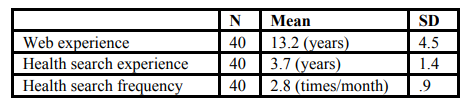
\includegraphics[width=0.8\textwidth]{Capture1.png}
	\caption{Consumers experience with web search and health search\label{fig1}}
\end{figure}  

Participants’ perceptions of the task seeking treatment options for migraine are shown in Figure~\ref{fig2}.

\begin{figure}[b!]
	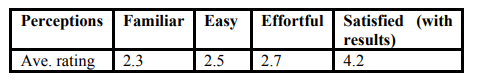
\includegraphics[width=0.8\textwidth]{Capture2.png}
	\caption{Participants’ perceptions of the task \label{fig2}}
\end{figure} 

According to these observations, participants have found that the task for searching treatment options for migraine to be somewhat familiar, somewhat difficult, needed a medium amount of effort on the task and have been generally satisfied with the results of the task. 

\textbf{Search Behaviour}

Search behaviours have been examined using the factors, such as session length, basic query behaviour and websites visited.

\textbf{Session length:} On average the session length to complete the task for searching migraine treatment options has been 10.25 minutes

\textbf{Basic query behaviour:} on average the number of queries that has been used to complete the task has been 4.2. The average query length has been 3.8 terms. Even though sometimes participants have had misspelled the term migraine as ‘migrain’ it has been easy to correct it with the use of the automatic suggestions.

Websites visited: The names of the websites that participants visited and the frequency of visits are shown in Figure~\ref{fig3}. It has been noticed that participants have frequently visited a set of medical-specific websites, such as WebMD, livestrong, mayoclinic, migraines.org and migraines.com, and a set of general-purpose sites, such as ehow, buzzle.com and Wikipedia which has made up approximately 60\% of all visits. Participants have also shown a checkout behaviour in several sites which has included medical-specific sites, evidence-based sites and general-purpose sites, and is reported as 73.2\% of all the visits. When considering sites which have been visited twice, half of them have been general-purpose sites and other half has been medical-related sites. The other category in Figure~\ref{fig3} represents 44 unique websites which have been visited only once. 

\begin{figure}[t!]
	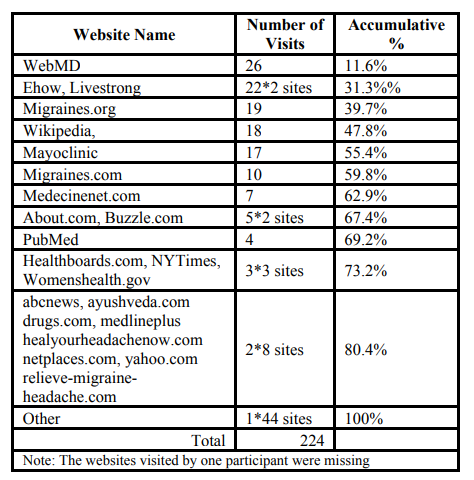
\includegraphics[width=0.8\textwidth]{Capture3.png}
	\caption{Websites visited during search \label{fig3}}
\end{figure}   

\textbf{Cognitive activities}

Cognitive activities have been analysed from four aspects:

(1)	query formulation and reformulation
(2)	examination of search results
(3)	judgment of sources
(4)	the development of cognitive activities over time
    
1.	Query formulation and reformulation

Types of query reformulations are shown in Figure~\ref{fig4}. According to these observations, participants have reformulated queries 89 times. Out of the different types of query reformulations, the three types which are switching to a new concept, paralleling moving between concepts (replacing a concept in the previous query to make the current query partially overlap with the previous one) and making a query more specific have had approximately equal number of reformulations. 

\begin{figure}[t!]
	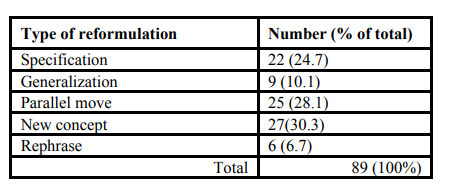
\includegraphics[width=0.8\textwidth]{Capture4.png}
	\caption{ Query reformulations\label{fig4}}
\end{figure}

2. Selecting search results 

According to the results observed, participants have preferred to perform a trial and error approach in order to provide a clear opinion about the search results (to select a search result or not). Other than that it has been noticed that the rank of the result has influenced participants when selecting a search result. This is because they have thought that results with high ranks are more relevant. 
  
Familiarity of websites has also been noticed as one factor which influence the selection of results. The reason has been because it brings comfortableness. 

The comparison of multiple sources in order to validate information found has been identified as another factor that influenced selection of search results.        

3. Judgment of sources

Participants have evaluated sources based on several criteria, such as design, readability, completeness, and credibility. However, relevance has not been mentioned by the majority of the participants because they have assumed that relevance is a necessary condition for a website to be appeared on the search results list. 

When considering the design, participants have preferred for clarity, simplicity, and clean design of websites (search interface and specific webpages). According to the participants, clean and well-structured design is helpful for them to find information easily and will increase the usability of the websites. Therefore, they have preferred to have breaking up of text, having images and diagrams in the website content. 

When considering readability participants have stated that they do not like to have technical language or “jargon” in the text content. 
 
Completeness of information has also been another important factor when judging sources because some participants have preferred to have both pros and cons for a particular treatment with the explanations of them.  
Various aspects of treatments, such as side effects and the expensiveness have also been required by some of the participants to judge the information sources.
  
When considering credibility, the participants have required to have credibility depending on their experience and the content of the website. 

4. Search timeline - Cognitive development

When considering the search timeline, there have been several patterns. 

One pattern is that participants starting from general or broad information and then gradually seeking for more specific information. Therefore, at the prime state the participants’ focus has been on general or broad information. Later in the search timeline the participants have tended to seek for more specific information. 

Another pattern is that participants starting from confirming information and then gradually seeking for novel information which has ended with validating the information for some participants. Participants have preferred to confirm their information because it makes them comfortable with the information. In the middle of the search timeline the participants have tended to seek for novel information which give them the opportunity to learn new factors. Finally, at the end of the timeline participants have preferred to do a final validation of the information that they have found. For example, one participant has revisited a website at the end of search process when he/she has wanted to double check to see whether a side effect was remembered correctly. In another example, a participant has revisited websites at the end of the search process to make sure that he/she has not missed anything.      

\textbf{Discussion}

When considering the first research question which is ‘what behaviours do consumers exhibit when they search for treatment options online?’, the main behaviours which could have been identified were consumers submitting short queries, misspelled keywords, and selecting results exclusively from the first page of search results. 

When analysing the websites, the participants have visited, firstly, the researchers have been able to notice that 30\% of the websites have accounted for 80\% of the visits made by the participants. Secondly, researchers have noticed that even though the majority of the websites the participants have visited was medical-specific sites, the participants also have relied heavily on general websites (30\% of the visits). The reason for this may be because of the higher rank of the websites, such as Wikipedia and the higher understandability of the text content. However, evidence-based trustworthy sources, such as MedlinePlus and PubMed have been visited very rarely by the participants accounting for just 4\% of the total visits. Finally, it is said that consumers are tend to visit websites when a site’s name contains the medical condition that they seek for. For instance, in this study 20\% of the 66 unique sites visited by the participants contained the term “migraine”.  

When considering the second research question which is ‘what cognitive activities are involved when consumers search for treatment options?’, the first aspect which has been evaluated was query formulation. The results indicate that consumers start searching for treatment options with general concepts and gradually focus on different treatments one after the other while exploring different aspects of each treatment.
 
When selecting search results, familiarity has been taken into account by the participants because the trustworthiness of such websites are considered as high. Credibility has not been considered very important may be because of the reason that participants’ intention has been to search for basic information just to get familiar with treatment options via search engine and rely on other sources, such as doctors to make final decisions.

When considering consumers’ cognitive development throughout the search process it is noted that they start by searching for general information and gradually move on to search for more specific information related to different aspects of a treatment. Also, another approach is to firstly search for more familiar information, then search for novel information and finally validate the novel information that has been found. Therefore, according to the observed search timeline information it is suggested that search engines need to accommodate such behaviours during a search. 

\textbf{Limitations}

1.	The task is a simulated task and do not reflect the participants’ real needs

2.	Due to the exploratory nature of the study, only one treatment option task has been assigned to the participants, thus participants’ behaviour may be affected by the nature of the task 
     
3.	A lab setting is not a natural environment for treatment search
    
\textbf{Conclusion}

Search behaviours of consumers’ when searching for treatment options are issuing short queries with misspellings and checking out only top results. Even with a timeline short as 10 minutes some consumers are tended to search information for confirmation and to obtain novel information. Search engines need to be designed so as to support consumers’ behaviours, such as searching to learn and confirm knowledge, rather than just displaying a set of popular results. For instance, it is necessary to present sites to consumers which contain complete and specific information, so that consumers are able to complete their searches more successfully. 
  
Consumers care more about the search engine ranking and the familiarity of the sites when selecting sources rather than the trustworthiness or usefulness of the information contained in the websites. Therefore, this shows that consumers are tended to use information sources with high ranks and are familiar to them no matter in which quality level (high or low) these sources are in.  

\section{Keselman, A., Browne, A. C., \& Kaufman, D. R. (2008). Consumer health information seeking as hypothesis testing. Journal of the American Medical Informatics Association, 15(4), 484-495.} 

It is said that consumers face a lot of difficulties when they search for health-related information online, for instance, when searching for self-diagnostic information in the absence of guidance from a health-care professional. Two of the main reasons for this are the lack of domain knowledge and less support provided by systems. Therefore, it is crucial to understand the process which is followed by consumers when searching for health information, in order to identify difficulties that they encounter. Hence, the objectives of this study have been to understand the most common patterns consumers follow depending on their initial theories and search strategies, and then to categorize the patterns as successful or failed. The importance of understanding the nature of consumers’ search challenges is that this information is vital in order to develop effective consumer health information resources which will eliminate these problems.  

In this study the researchers have proposed a framework that:

1.	‘Reconceptualises the iterative cycles of information seeking as attempts to verify or reject a pre-existing theory’

2.	‘Integrates stages of the information-seeking process with hypothesis testing’

In this framework there are several states which have been considered:

\textbf{State 1:} Beginning state which constitutes of the background knowledge (theory) and initial hypotheses (perceived information need)

\textbf{State 2:} Search goal

\textbf{State 3}: Shaping the search goal by search action steps

\textbf{State 4:} Evaluation of retrieved information

In a situation where it fails to “reconcile” the data with the theory, the theory revision has been made.
Also, because the framework used here has been a combination of a hypothesis testing perspective and Human Computer Interaction (HCI) perspective, it has been expected to obtain provide additional insight into consumers’ difficulties in locating and interpreting health information. 

The combination of hypothesis testing with Human Computer Interaction approach is shown in Figure~\ref{fig5}  

\begin{figure}[t!]
	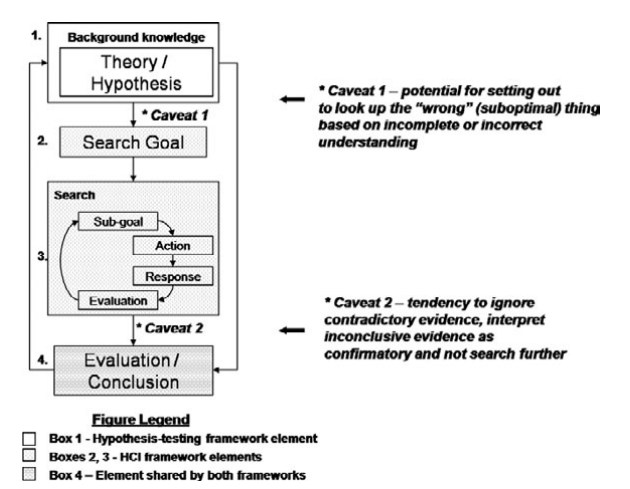
\includegraphics[width=0.8\textwidth]{Capture5.png}
	\caption{The combination of hypothesis testing with Human Computer Interaction approach \label{fig5}}
\end{figure}

 
This hypothesis-testing approach to information-seeking points out two potential pitfalls of the searching process:

1.	Knowledge-based hypothesis (hypothesis-testing framework) has the ability to influence the search goal (HCI framework), where an incorrect hypothesis may lead to searching irrelevant resources

2.	When evaluating retrieved information, prior hypothesis and background knowledge structure influences (affect) evidence interpretation

This framework has also linked information seeking with comprehension, which is considered as another core competency for utilizing health information effectively

\textbf{Methodology}

Twenty lay individuals have participated this study. For 10, the level of educations has been high school. The other ten has consisted of one with a Bachelor’s degree, seven with Master’s degree and two with doctoral degrees. 

\textbf{Procedure:}

Participants have been presented with a hypothetical scenario which describes symptoms typical of ‘stable angina’. Participants have been instructed to do two tasks:
  
1.	Semi-structured interviews: Discussed possible causes of the symptoms

2.	Search MedlinePlus: Seek information on the disease presented in the scenario

The semi-structured interviews have been audio-recorded. The search process has been recorded with TechSmith Morae® screen capture and video-analysis software. 

\textbf{Data Analysis:}

Information seeking processes’ information and semi-structured interviews’ information, such as participants’ theories about the causes, condition and severity of the situation described in the scenario, has been analysed separately. 

\textbf{Analysis of Semi-Structured Interviews - Participants’ Background Knowledge vs. Reference Model}

The information gained form the semi-structured interviews have been coded via semantic analysis. Then the completeness and the connectedness of participants’ knowledge has been compared with a reference model of stable angina which has been represented in consumer health materials. This reference model has been able to identify core concepts which explains the condition and specified semantic relationship among concepts.

The process of extracting the reference model’s concepts and relationships from the consumer health texts is shown in Figure~\ref{fig6}

\begin{figure}[t!]
	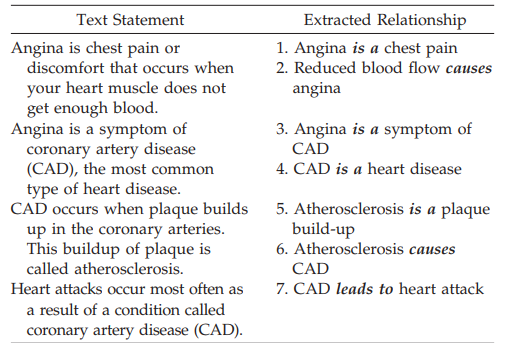
\includegraphics[width=0.8\textwidth]{Capture6.png}
	\caption{Converting Consumer Health Text into a Reference Model\label{fig6}}
\end{figure}

This reference model has linked three key concepts implicated in the scenario which are a physiological process (atherosclerosis), a resulting disease (coronary artery disease, CAD) and its primary symptom (stable angina chest pain). In addition, the model has also consisted of the concept of heart attack which is a condition that can be possibly occur due to coronary artery disease (CAD) progression. Furthermore, the model has been consisted with a general concept of heart disease encompassing both CAD and its potential outcome, heart attack. The five symptoms from the hypothetical scenario (chest pain, neck pain, shortness of breath and nausea) have also been clustered as manifestations of a single, diagnostically significant problem. 

Since the reference model has been based on consumer related materials, it has been represented as a simplification of the problem rather than including health-professional related terminology.

The reference model which has been used in this study is shown in Figure~\ref{fig7}

\begin{figure}[b!]
	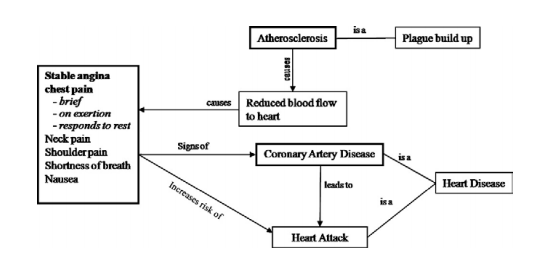
\includegraphics[width=0.8\textwidth]{Capture7.png}
	\caption{The Reference Model\label{fig7}}
\end{figure}


\textbf{Analysis of Information Seeking—Hypotheses, Search Goals, Search Actions, and Information Evaluation}

The searching process has been analysed using a software known as QSR NVivo. Using this software the data segments have been labelled with descriptive coding categories. Then the researchers have searched for patterns among these categories. Each searching processes’ data has then been labelled with two types of codes, such as action-related codes and competency codes. These search process recordings have been integrated with the verbal transcripts obtained during semi-structured interviews of each participant. This has been helpful because it has allowed researchers to closely monitor participants’ behaviour by comparing each action with the verbal transcript. With the NVivo analysis of the resulting protocols (combinations of search process recordings and verbal transcripts), researchers have been able to examine search strategies and visualize trends across participants’ behaviours.   

\textbf{Action-related codes:}

Represents steps of information seeking cycle. These steps are shown in Figure~\ref{fig8}. According to the framework of this study information seeking process is decomposed into a number of ‘iterative goal-action system response cycles’. These steps have also been expanded using sub-codes which are related to the primary hypothesis-testing and evidence evaluation.    

\begin{figure}[t!]
	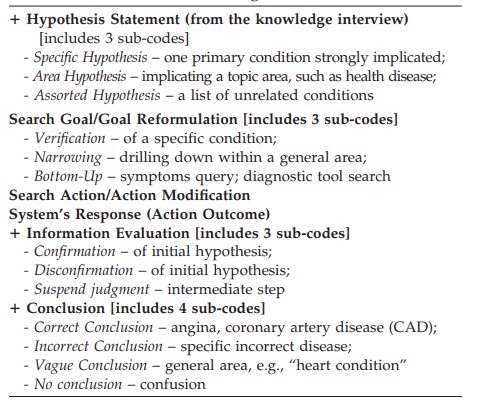
\includegraphics[width=0.8\textwidth]{Capture8.png}
	\caption{Information Seeking Codes\label{fig8}}
\end{figure}

Then participant’s information seeking path has also been graphically represented as series of states and actions. 
  
Based on this information and participants’ information seeking paths, the researchers have been able to identify a set of common information-seeking and reasoning patterns. 

\textbf{Competency codes:}

In order to characterize the role of participant competencies researchers have modified the scheme so as to include:

• Domain Knowledge (e.g., of heart disease) 
• General Search Strategies (e.g., query expansion) 
• Resource Knowledge (of MedlinePlus®) 
• Metaknowledge (of desirable site characteristics) 
• Language (spelling and vocabulary knowledge) 

These competency codes have been assigned to specific action steps which have been made during the information seeking process. For example, a competency code has been assigned to a statement which says that MedlinePlus health topic pages had a Diagnosis section, as representing Resource Knowledge competency.

\textbf{Results}

\textbf{Participants’ Demographics and Characteristics}

According to the observations females have reported as frequently using the Internet to obtain health information than males. The observations are shown in Figure~\ref{fig9}

\begin{figure}[b!]
	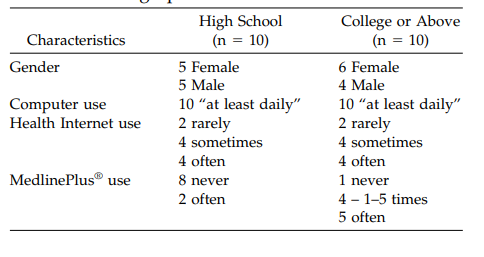
\includegraphics[width=0.8\textwidth]{Capture9.png}
	\caption{Demographics and Characteristics\label{fig9}}
\end{figure} 

\textbf{Participants’ Models of the Scenario: Background Knowledge and Hypotheses}

On the surface level, participants’ understanding of the scenario is identified as incorrect or imprecise

•	Seven participants: ‘The symptoms described in the scenario most likely signified a heart attack or a potential heart attack’ 
•	Eight participants: ‘The person in the scenario suffered from some “heart problem”’
•	One participant: ‘Old age’
•	Four participants: ‘Listed a number of cardiac and non-cardiac (e.g., stroke) illnesses that could explain the symptoms in the scenario’ 

When participants understanding of the scenario has been compared with the reference model, researchers have found that participants’ understanding is differed from the reference model in three critical aspects which are key concepts, symptoms’ grouping and symptoms’ characteristics. 

\textbf{Key concepts}

Two (coronary artery disease (CAD) and angina) of the three disease key concepts of the reference model have not been mentioned by the participants. Instead of the third key reference model concept, atherosclerosis, the lexical form of the term has been mentioned by only 3 of 20 participants and 18 have made some reference to the blockage of blood vessels

For 19 of the participants, cardiac concepts have been prominent in their explanation of the disease

18 Participants: Have mentioned heart attack either as their primary hypothesis or as a candidate hypothesis
 
‘Blockage of blood vessels’ has been identified as a main mechanism for causing cardiac problems

Other mechanisms: Tear to the heart muscles, irregular heart beat and “electrical problem with the heart”

Eight participants: Have suggested that the symptoms could be related to non-cardiac problems, such as stroke, arthritis, asthma and diabetes, but have not been always supported by a physiological explanation  

\textbf{Symptoms’ grouping}

According to the reference model all symptoms in the scenario are potential indicators of one condition. However, according to participants’ models, nausea and dizziness have been seen as unrelated to a cardiac problem, and indicative of a co-occurring non-cardiac condition

\textbf{Symptoms’ characteristics} 

None of the participants have noted the significance of the short duration or pain, its relation to exertion and response to rest which has been identified in the reference model. 

It has also been noticed that according to the language used by participants in their discussions, participants have lack of medical vocabulary knowledge. In some cases however, partiicipants have become aware of the fact that the scenario did not conform to classic symptoms of a heart attack and therefore, have used terms, such as ‘potential’ in their explanations. 

\textbf{Information-Seeking Processes: Goal Setting, Search Execution and Information Evaluation}

Because it is suggested that information seekers’ search goals are influenced by their prior knowledge and according to the observations of participants’ knowledge, it is suggested that for many participants, their initial search goals will not directly involve angina or coronary artery disease (CAD), instead the search goals will include cardiac problems.    

In this study researchers have partitioned the data on the basis of the initial search goals and moves instead of hypotheses and then they have related patterns or knowledge used for these trajectories. It has been noticed that initial action performed in each case is consistent with the expressed search goal. Therefore, the participants have been categorized into three main clusters, such as Verification-First, Problem Area Search-First and Bottom-Up. 

Key statistics for each cluster is shown in Figure~\ref{fig10}

\begin{figure}[t!]
	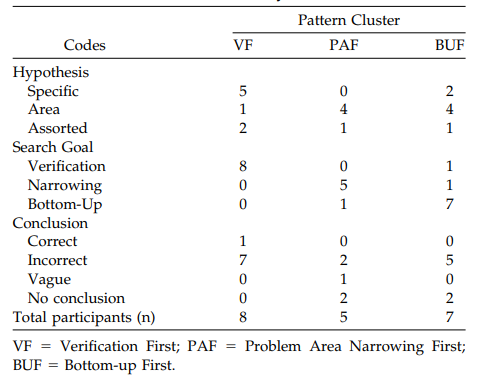
\includegraphics[width=0.8\textwidth]{Capture10.png}
	\caption{Key statistics for each cluster\label{fig10}}
\end{figure}

\textbf{Verification-First Cluster}

Has included 8 of the participants (40\%). These participants have started the search process by attempting to verify a specific illness. Therefore, they have started out with a specific hypothesis which is ‘a heart attack’. All the other hypothesis of this cluster also have been related to heart attack. At the beginning of the search all participants have been navigated to a high-quality heart attack site. The only strategy which has been used in this cluster has been ‘verification’. 

Seven participants have incorrectly concluded that the situation described in the scenario involves heart attack by only considering the similarities between descriptions of heart attacks and symptoms in the scenario, such as squeezing chest, neck and shoulder pain, shortness of breath and nausea. They have ignored the differences, such as symptoms in the scenario emerged upon exertion, lasted 2–3 minutes only, and can be alleviated by rest. 

Also, because the researchers have noticed differences in ‘symptoms’ characteristics’, in participants’ models and the text-based reference model, it is said that this behaviour of ignoring symptoms’ characteristics that are viewed as non-essential, can be seen as exemplary of the ‘selective perception bias’. 

When considering reasoning patterns researchers have observed a ‘confirmation bias’. Participants’ of this cluster have tended start searching with heart attack hypothesis, then navigating to a heart attack related site and making conclusions that the information has confirmed their hypothesis. 

A ‘premature search termination bias’ has also been observed in some participants where they have stopped their search just after reviewing only one content topic because they have found that information to be satisfactory. 

However, one participant of this group has not followed the normal pattern which has been seen from other participants. This participant has noticed the differences in the duration of the symptoms in the scenario and of the symptoms of heart attack. Therefore, he has followed a link from the MedlinePlus heart attack encyclopedia page to the angina page and has concluded that the scenario described is angina. 

Information seeking sequences of verification-first participants is shown in Figure~\ref{fig11}

\begin{figure}[t!]
	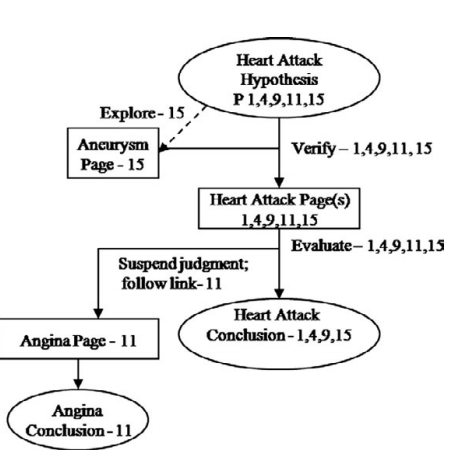
\includegraphics[width=0.8\textwidth]{Capture11.png}
	\caption{Information seeking sequences of verification-first participants\label{fig11}}
\end{figure}

\textbf{Problem Area Narrowing-First Cluster}

Has included 5 of the participants (25\%). These participants have started the search process with problem area search. Therefore, this group has been consisted with participants who have had ‘Area’ hypothesis and ‘Assorted’ hypothesis. For instance, some have started searching with queries, such a ‘heat disease’ and others have browsed the site index tree. Only one participant has switched to a ‘bottom-up’ approach during this searching process. They have also shown a behaviour of eventually navigating to sites which describe specific diseases. In contrast, to the verification-first cluster, participants in this cluster have tended to leave without a conclusion rather than providing incorrect conclusions. 

According to one participant’s behaviour in this group it is said that ‘selective perception bias’ can be seen in this cluster because this participant has concluded the scenario to be the patient having ‘very minor heart attacks’ and in the scenario it mentions as the pain episode only lasts 2–3 minutes. It is noticed that the ambiguity in the description of the scenario may also have lead participants in providing wrong conclusions. For instance, when it says ‘goes away and come back’ it is not clear from the text how long the period of recurrence is. 
     
The configuration of the web resources has also been identified as one of the reasons for the problems which have been faced by the participants. Even though many retrieved results for participant queries have consisted of links to relevant information about angina, these links have not been prominently displayed in the participants’ view. Therefore, some participants have not even realised that such choices were available to them. Some subtopics have been followed by a number of irrelevant subtopics and some relevant results have been displayed at the bottom of the screen which have been impossible to see without scrolling the page.   
  
Information seeking sequences of problem area narrowing-first participants is shown in Figure~\ref{fig12}

\begin{figure}[t!]
	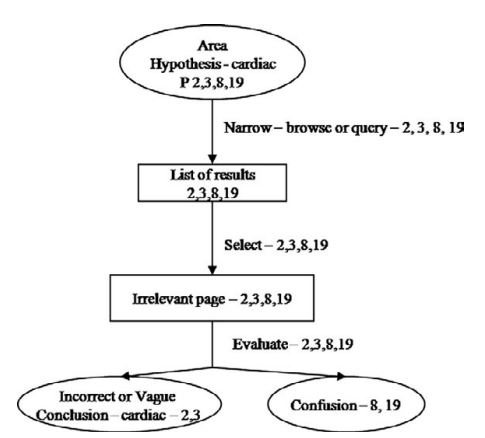
\includegraphics[width=0.8\textwidth]{Capture12.png}
	\caption{Information seeking sequences of problem area narrowing-first participants\label{fig12}}
\end{figure}

\textbf{Bottom-Up First Cluster}

Has included 7 of the participants (35\%). Some of the participants have started the search process without a specific hypothesis. A few others have found bottom-up strategy to be unsuccessful because they have attempted to search for a general-purpose diagnostic tool which has not been included in MedlinePlus. These participants have shown a behaviour where they have switched to other ‘hypothesis-driven strategies’, but have made incorrect heart attack conclusion. Even though the participants who followed the bottom-up strategy have progressed toward the accurate conclusion, neither of them have been able to make the exact correct conclusion as angina.  

As observed in the problem area narrowing-first cluster, even though the participants of this group has been able to retrieve relevant links, these links have been scattered throughout variably relevant subtopics and have been viewed at the bottom of the results page. One reason for this issue has been identified as the imprecise search strategies entered by the participants. 

Also, some participants have shown a ‘selective perception bias’ where they have tried to match description of a heart attack with the facts mentioned in the scenario. 

Early termination has shown to be less common when compared to verification-first cluster where only two participants have stopped their search after reviewing a single content webpage.  

Information seeking sequences of bottom-up first cluster participants is shown in Figure~\ref{fig13}

\begin{figure}[t!]
	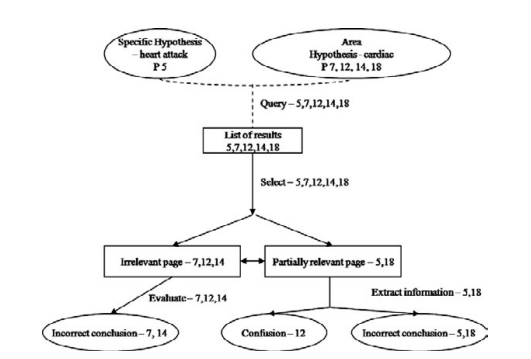
\includegraphics[width=0.8\textwidth]{Capture13.png}
	\caption{Information seeking sequences of bottom-up first cluster participants\label{fig13}}
\end{figure}

\textbf{Other Factors: The Role of Web Resources, Education Level and User Competencies}

According to frequency distribution of different kinds of qualitative competency codes, it has been noticed that different types of knowledge are instrumental during different search stages. Domain knowledge has been important for setting goals and information evaluation. Domain understanding has been important for determining the direction of the search and for the interpretation of the results. Resource knowledge, strategies and metaknowledge have been important for navigational actions. 

Excerpts of Coded Information Seeking Protocol of a participant is shown in Figure~\ref{fig14}

\begin{figure}[t!]
	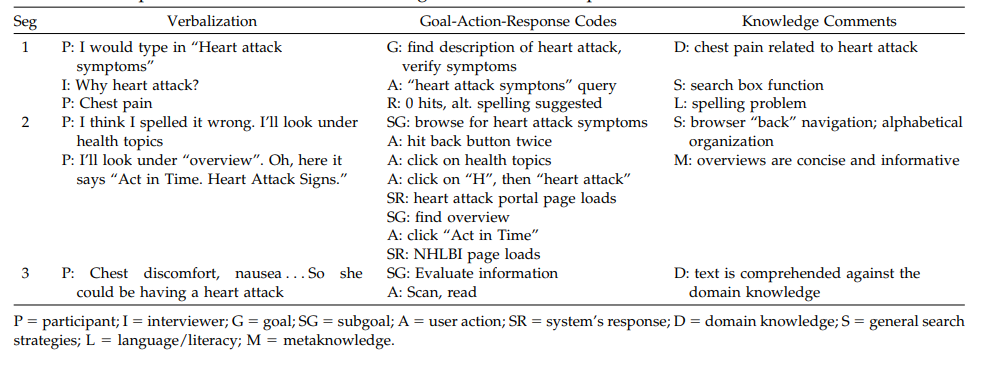
\includegraphics[width=0.8\textwidth]{Capture14.png}
	\caption{Excerpts of Coded Information Seeking Protocol of a participant \label{fig14}}
\end{figure}

Information seeking competencies have been differentially impacted by the levels of education. Despite of the level of education participants have demonstrated comparable levels of understanding of the symptoms described in the scenario (domain knowledge). In addition, it has been noticed that participants with higher levels of education are likely to be familiar with MedlinePlus, have used efficient search strategies and are tended to make meta-level comments, such as judging the authoritativeness of a source. However, incomplete and inaccurate domain knowledge has led participants to apply their efficient strategies to the wrong pages and this has also made participants ignore some key aspects of the information. 

Lack of medical vocabulary knowledge has been observed as an additional challenge to the participants. They have lacked precise labels to explain their concepts. Because of this knowledge gap some participants have not been able to use relevant terms when formulating their queries and have not recognized such term while scanning topics or lists of results. For instance, some participants have read the term “angina” in index trees, but have not perceived it as relevant. Participants with high school education have been identified to be affected the most by vocabulary-related difficulties.   
        
Two aspects of the MedlinePlus interface have also been identified as influencing participants’ search process. The first aspect has been the ‘lack of explicitness in relating lay and professional terms in the index’. For instance, it is said that in the alphabetical list of topics, the Chest Pain title suggests the topic Angina, but the Angina title does not suggest the topic chest pain. The second aspect has been about the order and organization of query results lists, because it has been noted that some relevant links have been presented after general/ less relevant links.   

\textbf{Conclusion}

Usually when individuals search the web for information in the absence of a diagnosis, they are unable to reach pages with relevant or needed information. 

When compared with the participants in cluster 1, participants in other two clusters have shown a behaviour to terminate their search before reaching a conclusion.  If a participant start the searching process with a specific preconception of what the answer might be, they are more likely to leave satisfied but with incorrect beliefs which match their initial hypotheses. On the other hand, if the participants do not have a specific preconception of what the answer might be, then they are more likely to leave without any conclusion.   
Gaps in health-related knowledge have an impact when reasoning information. 

The framework used in this study has suggested that the influence which is made by prior knowledge should be monitored throughout all stages of information seeking. In addition, hypothesis generation and information evaluation have been considered as two points where prior knowledge is more likely to lead to sub-optimal choices and biased reasoning strategies. 

Also, domain knowledge has been identified as important when setting information goals and evaluating retrieved information. Efficient search skills, internet experience and education level are not able to compensate the lack of domain knowledge. 

When analyzing participants’ information-seeking patterns, researchers have identified several cognitive biases, such as confirmation bias, selective perception, and premature termination of search for evidence. These cognitive biases are said to be particularly relevant when gathering evidence and generating knowledge.  

The importance of identifying the difficulties faced by consumers’ is that health information website(consumer health sites) designers can try eliminate these difficulties by providing support in places where consumers are tend to behave erroneously. Such support can be provided at three levels, such as in information portals like MedlinePlus, in individual websites and education tools. In information portals query suggestions can be made to make the consumers’ queries more specific and information can be presented in a way which will emphasize alternatives so as to facilitate hypothesis testing. Also, they can facilitate in suggesting consultation with a health professional. In individual websites needs of targeted users can be addressed. In all of these levels it is important to have consumer-friendly terminology with consumer-friendly definitions. These terms then can be explicitly linked to professional terms. In education tools consumers can be taught how to formulate specific queries, to evaluate qualifiers in the information and to not terminate their searches prematurely. 

The characteristics of this research situation: the hypothetical nature of the scenario, which may have affected the users’ motivation, the complexity of the diagnostic task and the similarity between angina and heart attack symptoms have also been identified as potential reasons which have led this study to result in a very low success rate. 

\section{Zhang, Y., Wang, P., Heaton, A., \& Winkler, H. (2012, January). Health information searching behavior in MedlinePlus and the impact of tasks. In Proceedings of the 2nd ACM SIGHIT International Health Informatics Symposium (pp. 641-650). ACM.} 

Searching for health information online by consumers has been identified as the third most popular online activity. The aim of this study has been to investigate consumer health information searching behaviour (interaction behaviour) in web. Therefore, the researchers have observed consumers’ health information searching behaviours in MedlinePlus. They have also examined to identify whether there is any impact on the search behaviours, by the number of concepts involved in search tasks. The research questions of this study have been:

1.How do users search MedlinePlus? 

2. How do users browse MedlinePlus? 

3. How do search tasks influence interaction strategies? 
     
In addition, by examining the search processes and strategies, the researchers also have aimed to understand difficulties faced by consumers while searching in MedlinePlus and how they handle these problems.  

\textbf{Methodology}

Twenty undergraduate students (11 females and 9 males) have been recruited for this study who have not used MedlinePlus prior to this study.

MedlinePlus: Is a system which provides free and trusted consumer health information to the public. This system contains information, such as publications of medical research, licensed medical dictionaries, encyclopedia, prescription drugs and directories of health professionals and hospitals. At the time of this study, MedlinePlus has been a browsing oriented system with a simple search engine. In addition, the homepage has also listed major information sources, health topics, encyclopedia and dictionary.  

\textbf{Search Tasks}

Each participant has been instructed to perform three search tasks based on the given scenarios.Task 1 related to finding arguments 'for and against the use of marijuana for medical purposes', Task 2 related to finding 'the relation between Type I and Type II diabetes, and hypertension' and Task 3 related to 'finding the functions of liver and kidney, what is the role of insulin in the liver and kidney, why insulin would be needed? and whether insulin is related to liver and kidney diseases?'.

\textbf{Procedure}

Prior to conducting the tasks, participants have been instructed to complete a 'ETS VZ-2 paper-folding test' which measures their spatial ability and to complete a demographic questionnaire which represents each participant's major field of study, computer experience and medical information searching experience. After giving some time to explore MedlinePlus, the participants have been instructed to complete the three tasks by taking as much time they needed. At the end of each task participants have been instructed to rate the difficulty of the task, required mental effort and satisfaction of the search performance. All the search session have been video captured using 'Camtasia' software. At the end of all searching tasks participants have been interviewed in order to gather information, such as impressions towards the tasks, the MedlinePlus website and each search process. 

\textbf{Data Analysis}     

Types of data collected:

1. Demographics and spatial ability
2. Video-recordings of search sessions
3. Interviews

Each webpage has been considered as an analytical unit and when navigating to a new webpage one record has been created. All the actions performed on a webpage (clicks and issuing queries) have been transcribed and incorporated with the record. 

In addition, all the queries issued have also been transcribed. In cases where participants reformulated the queries, the actions performed to reformulate the queries, such as adding a concept and deleting a concept have been identified in order to analyse query reformulation. Furthermore, different conceptual changes have also been identified and examined. In order to perform this query reformulation analysis, the researchers have adopted a coding schema for query reformulation. Then the researchers have also expanded this schema in order to include new types of conceptual changes which arises from the data collected in this study. Each instance of query reformulation has been considered as a unit of analysis when analysing both actions and conceptual changes.        

In order to analyse participants' interaction strategies, searching and browsing behaviours have been considered. 

Searching: Issuing a query to MedlinePlus website via the search box

Browsing: Following a sequential paths/links while seeking for information. 

In addition, other different sequential transitions, such as searching to searching, searching to browsing, browsing to browsing and browsing to searching have also been considered when analysing participants' interaction strategies.     	
	  
Information obtained via interviews have been analyzed using open coding method.

\textbf{Results}

\textbf{Participant characteristics}

For 19 of the participants:

Spatial ability score range: 6.8 to 17.6
Age range: 18 to 21 years
Internet experiences range: 6 to 13 years

Searching medical or health-related information online: 19 participants have searched medical information online on a yearly or monthly basis using sources, such as general web search engines and health information from university website 

\textbf{Session length and perception of tasks}

Session lengths: Lasted between 11.63 to 29.01 minutes

Time spent on each task and other perceptions, such as the difficulty, mental effort and satisfaction are shown in Figure~\ref{fig15}

\begin{figure}[t!]
	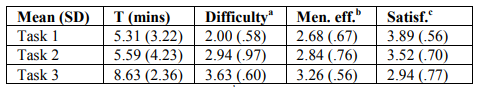
\includegraphics[width=0.8\textwidth]{Capture15.png}
	\caption{Time spent on tasks and perceptions of the tasks \label{fig15}}
\end{figure}

Time spent for Task 3 has been identified as significantly higher than Task 1 and Task 2. The time difference for Task 1 and Task 2 have been noticed as not statistically significant. 

Task 3 has had the highest difficulty followed by Task 2 and Task 1. The highest mental effort has also been required for Task 3 according to these results, but again Task 1 and Task 2's difference in mental effort has been identified as not statistically significant. Participants have been least satisfied with Task 3 and the difference in task satisfaction for Task 1 and Task 2 has been identified as not statistically significant.

\textbf{Search behaviour}

Search behaviour has been analysed using four aspects:

1. Query features
2. Search terms
3. Query reformulation
4. Access to results

\textbf{1. Query features: number of queries and terms}

The number of queries and query terms for each task are shown in Figure~\ref{fig16}

\begin{figure}[b!]
	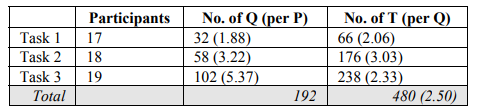
\includegraphics[width=0.8\textwidth]{Capture16.png}
	\caption{Query features: number of queries and terms \label{fig16}}
\end{figure}

The difference between the number of queries which have been issued during each task have been identified as statistically significant with Task 3 having the maximum number of issued queries and Task 1 having the minimum number of issued queries.

Average query terms has been 2.5 with Task 1 having the shortest queries and Task 2 having the longest queries, but the difference has been identified as not significant. 

\textbf{2. Search terms}

There have been three types of search terms:

1. Keywords with semantic meanings (meaningful terms): represents participants' understanding of the tasks. Have been taken from task descriptions and synonyms have also been used. For instance, 'high blood pressure' has been used as a synonym for 'hypertension' in Task 2.

2. Stop words (No semantic meaning): To connect query words
3. Search operators (AND, OR)

Search terms for each task are shown in Figure~\ref{fig17}

\begin{figure}[t!]
	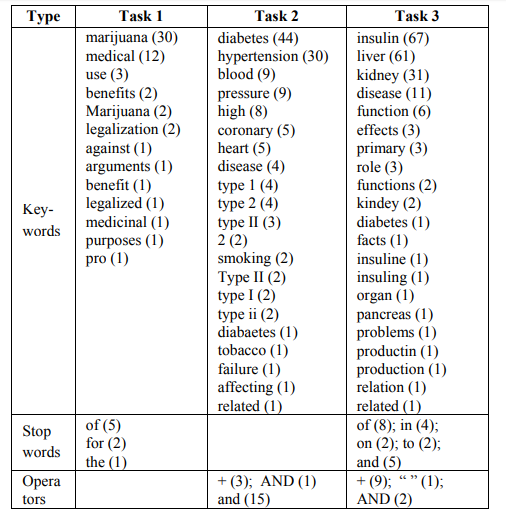
\includegraphics[width=0.8\textwidth]{Capture17.png}
	\caption{Search terms \label{fig17}}
\end{figure} 

Some participants also have searched for new concepts associated with the concepts mentioned in the scenarios. For instance, searching for 'heart failure' in Task 2 which is related to hypertension. This behaviour has been identified in people who have been more aware of the scenario explained depending on their personal knowledge and experiences.

The use of stop words have demonstrated that participants are tended to use natural language during search. 

\textbf{3. Query reformulation}

Query reformulation analysis is important to understand changes to participants' perceptions of the tasks and changes to their mental models of the system during the searching. This analysis has been performed based on:

1. Executed actions which modified the initial queries

2. Subsequent conceptual changes to the queries

\textbf{Executed actions which modified the initial queries}

Three actions have been identified;

1. Concept related changes: Add, delete, repeat and change to a new concept

According to the data collected for this study, researchers have noted five different patterns of actions, such as  adding concept(s), deleting concept(s), replacing concept(s), repeating concept(s),
and changing to new concept(s) that are not included in the previous query. 

In total,

30\% query reformulations: Replaced concepts in the previous query with a new concept

28.9\% query reformulations: Added concepts to the previous query

20.7\% query reformulations: Changing to new concepts that are not appeared in the previous cycle

Repetition of previous query has not been performed very frequently

Task 3 has had the maximum number of query reformulations and has involved more patterns of action.  


2. Form of terms (singular and plural)

Two actions have been performed to change the form of the terms. First action is the change to the form of the term, such as changing 'type ii diabetes' to 'type 2 diabetes'. The second action has been to correct the misspelled terms, such as correcting the term 'insuling' to 'insulin'. 

3. Conceptual relationships (Boolean operators)

Changes done to the relationships among concepts, such as changing the query 'liver disease AND insulin' to 'insulin liver disease' by dropping the 'AND' term and altering the order of the words. 

\textbf{Subsequent conceptual changes to the queries}

Conceptual and semantic changes to queries which has been resulted from different actions performed on queries have been categorized into 4 sections of conceptual changes.

(1) Specification (the inquiry becomes more specific)

(2) Generalization (the inquiry becomes more general)

(3) Parallel movement (the reformulated query has a
partial overlap with the previous query; the two queries deal with somewhat different aspects of one concept)

(4) Replacement with synonym (replace the current terms with words with similar meaning): Synonyms have been considered as query iterations rather than conceptual changes

In cases where participants moved to new concepts which did not overlap with the previous query concepts, has been identified as 'switching topic'. 

In cases where participants re-executed the same previous query in order to get back to some results of that query has been identified as 're-execution'. 

In cases where participants made more than one change to a query in a single query reformulation, all the changes, such as replacing query terms with synonyms and making the query more specific have been counted and therefore, the total number of changes has been larger than the total number of query reformulations.

According to the results observed it has been identified that most of the query reformations are related to conceptual changes so as to make the subsequent queries more specific, followed by query reformations to make the subsequent queries more general,  to switch queries to a new topic and to make a parallel movement. When considering query iterations query re-execution has been performed more than replacing query concepts with synonyms.

Actions and frequencies related to query reformulation are shown in Figure~\ref{fig18}

\begin{figure}[t!]
	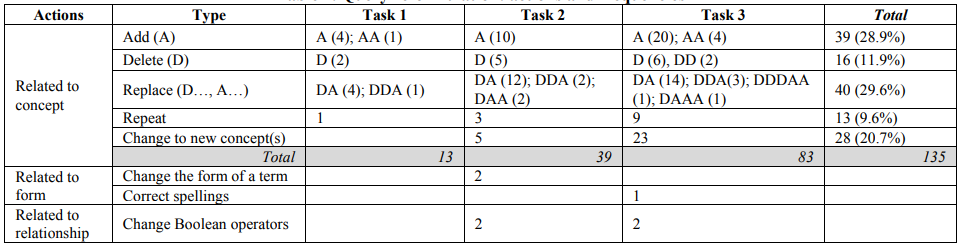
\includegraphics[width=0.8\textwidth]{Capture18.png}
	\caption{ Query reformulation: actions and frequencies \label{fig18}}
\end{figure} 

Semantic changes related to query reformulation are shown in Figure~\ref{fig19}

\begin{figure}[b!]
	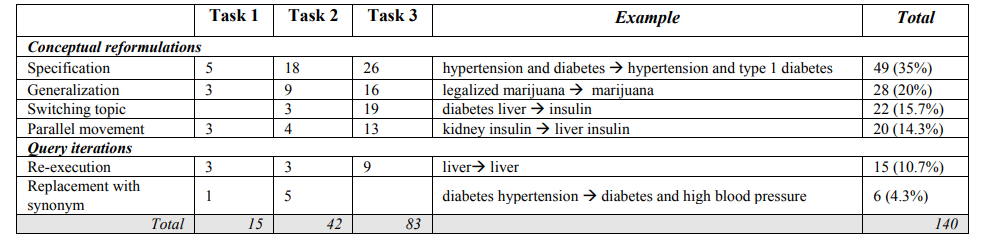
\includegraphics[width=0.8\textwidth]{Capture19.png}
	\caption{ Query reformulation instances: semantic changes \label{fig19}}
\end{figure}    

\textbf{4. Accessing and evaluation results}

Once the retrieved results are presented as a 'relevance-ranked list', participants have been given three paths to proceed.

1. To access documents from the result list
2. To limit displayed results to a particular section, such as health topics, external health links, and news (a filtering option provided by MedlinePlus)
3. To limit results to a particular topic cluster, which has been generated by the system based on the topic being searched (a filtering option provided by MedlinePlus)

According to the observed results, most participants have shown a behaviour to directly click on links rather than using filtering options provided by the MedlinePlus website. Therefore, 18 participants have clicked on direct links to 155 documents, 8 participants have used the collection option 31 times and 6 participants have used topic cluster option 7 times. Only 2 participants have accessed articles on second and third pages of the results.       

The evaluation of the results has been done by scanning the results lists and choosing links based on the keywords in the headings. Participants also have evaluated results based on facts, such as who is behind the information and how the content has been presented. Two participants have also evaluated the information in MedlinePlus as biased because the government provided much of information.  

\textbf{Browsing Behaviour}

Browsing is referred to as participants' behaviour of accessing different structures, such as alphabetical lists and subject hierarchies. Participants have shown this browsing behaviour when they have accessed a particular information resource type, such as encyclopedia and collections of health topics. 

\textbf{1. Accessing different resources}

MedlinePlus has consisted of two sections, such as 'Drugs \& Supplements' and 'Encyclopedia' which have been organized in alphabetical order. According to the results observed, 6 participants have accessed Drugs \& Supplements and 12 participants have accessed Encyclopedia via  the alphabetical lists. News section is another section which has been available on MedlinePlus and 1 participant has accessed this section. 

MedlinePlus has also contained a Health Topics section with 6 next level schemas, such as alphabetical list, body location/systems, diagnosis and therapy, disorders and conditions, demographic groups, and health and wellness. 13 participants have accessed Health Topics section. Also it has been noticed that the majority of the participants have accessed these schemas while performing Task 3. 'Alphabetical list' has been the most used schema (50\% of the usage of all schemas) and has been used by 7 participants. 'Body Location/System' has been the second most used schema (43\% of the usage of all schemas) where 12 participants have used it. The schemas 'Diagnosis and
Therapy' and 'Health and Wellness' have only been used by 1 or 2 participants.                 
 
Data related to accessing a particular health topic is shown in Figure~\ref{fig20}

\begin{figure}[t!]
	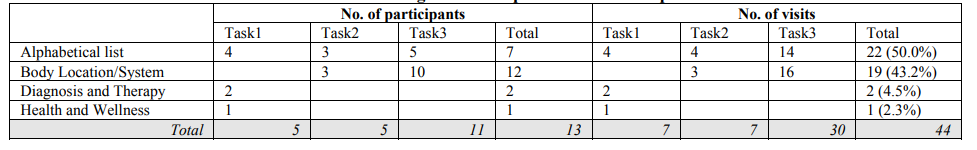
\includegraphics[width=0.8\textwidth]{Capture20.png}
	\caption{ Browsing to access a particular health topic \label{fig20}}
\end{figure} 

\textbf{2. Accessing related topics}

In MedlinePlus, health topic pages contain both in-text and related topics hyperlinks. These links can be used by participants to access additional resources. However, only 9 participants have looked for information using related topics links. Both the in-text and related topics links have been equally used specially for Task 3.   

Data related to accessing related topics is shown in Figure~\ref{fig21}

\begin{figure}[t!]
	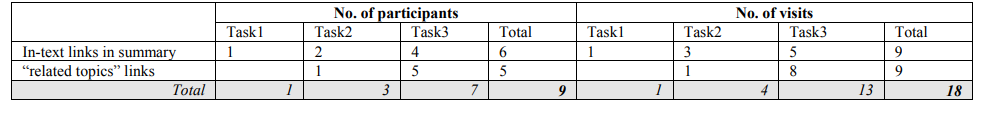
\includegraphics[width=0.8\textwidth]{Capture21.png}
	\caption{ Browsing to access related topics \label{fig21}}
\end{figure}  

     
\textbf{A Holistic View of Search Strategies}

MedlinePlus' information architecture supports for both searching and browsing. Therefore, information searching strategies in MedlinePlus include both  deployment of searching and browsing techniques, and selection and use of different types of resources. Hence, two aspects have been taken into account when analysing the strategies that participants have used for searching information in MedlinePlus. 

1. Use of resources

The Health Topics section has been identified as the most accessed resource because all participants have accessed at least one health topic page by selecting a link from the search results or by using browsing strategies. 

The medical encyclopedia has been the second most used source by participants where 13 participants have accessed encyclopedia by clicking the link in search results or by directly navigating to the source. It has also been noted that medical encyclopedia has mainly been used for Task 2 and Task 3.

Dictionary has also been accessed by 6 participants during Task 3.  

The Drugs \& and Supplements section has been accessed by 4 participants and has been used mostly for the Task 1. 

A very few participants have also accessed News, Directories, Go Local and Multiple Languages
sections of MedlinePlus.     

2. Use of searching and browsing strategies

In terms of searching participants have used the main site-wide search and they have also searched the Dictionary. In terms of browsing participants have browsed to access information in Health Topics (HT), Encyclopedia (E), Drugs \& Supplements (DS), News (N), and Related Topics (RT). It has also been identified that these two strategies have been used as a combination during the searching process.  
   
The sequences in which participants have used these strategies are shown in Figure~\ref{fig22}. The number of participants who adopted the sequence are also stated in the parentheses. 

\begin{figure}[t!]
	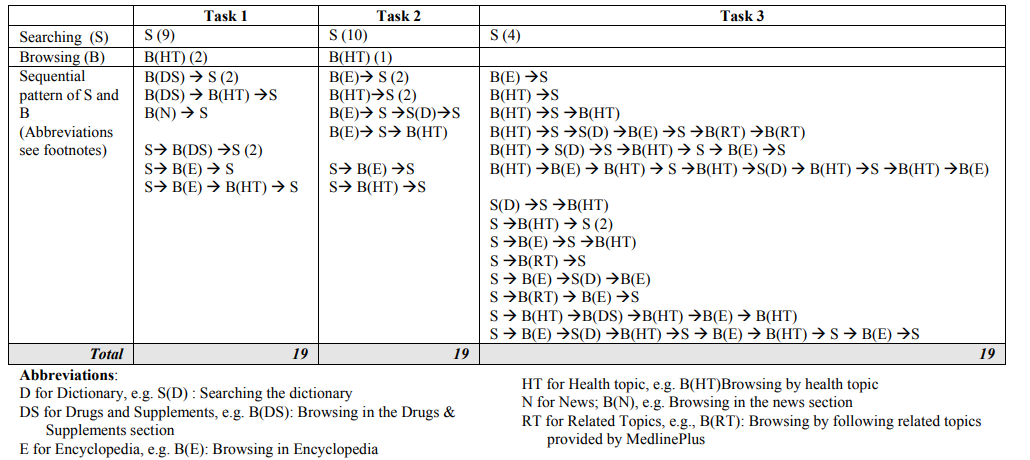
\includegraphics[width=0.8\textwidth]{Capture22.png}
	\caption{ Patterns of use of searching and browsing strategies in completing search tasks  \label{fig22}}
\end{figure} 

According to the results obtained, half of the participants have used only the 'searching strategy' for Task 1 and Task 2. A couple of participants have used only browsing for Task 1 and Task 2. When considering Task 3, 4 participants have used only searching and none of the participants have used only browsing to complete the task. 

When considering searching and browsing as a combination, 8 participants have used this combination to complete both Task 1 and Task 2. 15 participants have used this combination to complete Task 3.  

Therefore, the patterns in which searching and browsing have been deployed into the searching process, has been varied among the tasks. 

It has been noted that compared to Task 1 and Task 2, the patterns of Task 3 were more diverse, complex, exploratory, and iterative.

\textbf{Discussion}

The analysis in this study has been conducted using three main research questions.

1. How users search
2. How users browse
3. How tasks affect interaction strategy 

When considering how tasks affected interaction strategy, it has been noted that both browsing and searching strategies have been used to complete the three tasks of increased complexity as reflected by
conceptual multiplicity. 

According to the results observed, for the tasks with relative lower complexity, participants have tended to use either browsing or searching strategies to complete the tasks and searching has been the dominant choice. In cases where both the strategies have been used for lower complexity tasks, the interaction sequences have been identified to be short. For the tasks with relative higher complexity browsing has not been used alone.Long sequences of combined browsing and searching strategies have been used to complete this task.

Therefore, it is said that task complexity influences interaction strategies and pattern. However, overall participants have used searching strategies more than browsing. The reason for this is because when the descriptions are provided to participants, the effort is much less for the participants to enter search terms rather than to understand the classification underlying navigational paths which is required to perform browsing strategies. In addition, it has been noted that browsing strategies have been used by the participants to access the encyclopedia and dictionary to understand the concept and health topic in order to have a preliminary understanding of the questions before searching. 

Participants have used query terms from the task description and they also have used terms associated with the terms in the task description. The average query length has been 2-3 terms and participants also have made spelling mistakes in queries. Therefore, it is said that functions to detect misspellings and
make suggestions is needed when designing consumer health-related information websites.      

The mean session length has been identified to be in between 1.88 to 5.37 queries corresponding to complexity levels of the tasks.

When reformulating the queries, replacing concepts have been performed the most, followed by adding concepts and changing to new concepts. As a result, there have been two types of query reformulations namely, 'conceptual change' and 'query iteration'. In conceptual change', the meaning of the previous query has been changed. In 'query iteration', the meaning of the previous query has not been changed.

85\% of the query reformulation have been occurred as conceptual changes. Most frequent reformation type has been specification, followed by other types, such as generalization, switching topic, and parallel movement.                        
       	           
It is said that the higher number of query specifications and generalisations is due the difficulty that participants have faced when determining the level of specificity of the information needed. Therefore, the need of a hierarchical terminology structure has been identified to assist participants or users of the system in selecting query terms.

Switching topic and parallel movement have been identified as another two conceptual changes and occurrence of these changes are due to the exploratory nature of the tasks. 

It has been identified that MedlinePlus' support for exploring relationships between multiple conditions or health concepts, is limited. The lack of advanced search functions has also been noted by the participants.

Since backtrack function has not been available in MedlinePlus, participants have shown a behaviour to resubmit queries in order to generate the same results. Query resubmission is known as one form of query iteration. The other form has been replacing terms with their synonyms. According to the results it is said that general public have difficulties with medical
terminologies. 

According to the observations, the majority of the participants have accessed results by simply just clicking on the links in the results. Only a very few participants have used functions provided by MedlinePlus to limit the results to a particular type or subject. Also, some participants have tended to evaluate the quality of the results using certain criteria such as the source of the information. In addition, a very few participants have accessed links beyond the first result page.

When considering how participants browse, it has been identified that browsing has been performed frequently within  a sequence of both interaction strategies (browsing and searching). However, the links to related topics list and in-text links of summary have not been used much. 

When considering the high complex task, participants have shown a behaviour as to browse the Encyclopedia and Health Topics, or they have followed links to related topics in addition to searching.              

\textbf{Limitation}

1. Recruiting undergraduate students: Tends to have more versed skills in web searching but less often on health-related topics

2.  The tasks have been predefined rather than users’ real needs  

3. The information architecture and interface of a
web space can influence interaction behaviour. Therefore, it is valuable to observe the same user group using other consumer health information websites, particularly those with different structures to MedlinePlus

\textbf{Conclusions}

Searching strategies have been used more for the task involving three concepts than the tasks involving one or two concepts

Although reformulation of queries is identified as a strategy for retrieving better results, in this study reformulations have only been used as generalization or specification strategies. Therefore, they have been identified as moves along a conceptual hierarchy. 

It is said that synonyms and re-execution of previous queries should be improved by better design. Therefore, it is suggested that the systems to have automatic synonym expansions upon request and accessibility to search histories in order to  allow backtracking to a specific point of the earlier search results.

Browsing can only be performed successfully only if the users are familiar with the structure of the source or the terms given in task description. Therefore, most lay people are unlikely to be able to navigate through
MedlinePlus’s health topics due to the lack of medical conceptual structure. In order to solve this issue it is said that  the systems should design mechanisms to connect lay terms with medical terms.

The systems should be designed so as to have cognitive assistance to help users at different stages of a search. This would be really helpful for search tasks with varying complexity. For query construction, a display of terminological relationship has been identified as useful. For query reformulation, soliciting reasons can be used to suggest alternative moves. In addition, other improvements, such as adding advanced search features, making information architecture visible to users, and encouraging evaluation of search results can be incorporated with the new system designs. 

\section{Toms, E. G., \& Latter, C. (2007). How consumers search for health information. Health informatics journal, 13(3), 223-235.}

There is a rapid increase in the number consumers who search health information online. Therefore, in order to build better systems, it requires a holistic understanding of how health information consumers interact with online resources and the way they evaluate the retrieved results. Hence, the aim of this research has been to study the consumer health information searching  behaviour online in three aspects:

1. How people specify their information requests 
2. How people select from search result lists
3. How people examine the page(s) they declare relevant to the information search problem

\textbf{Methodology}

48 people have been recruited for the study.They have been instructed to perform the search tasks using Google. The data has been collected using several techniques, such as questionnaires,
transaction logs, screen capture and audio recording.  

\textbf{System used: Google}

For the purpose of this study the Open Directory categories have been added to the Google search engine page. Therefore, the participants have been instructed to enter their search or to select from the directory categories. Except that the standard Google interface screen has been retained. The purpose of adding the directory has been to provide the participants with an alternative option which is a scan capability.    

\textbf{Tasks}

Four tasks have been used in total and two tasks have been fully specified.

1. Find three categories of people who should or should not get a flu shot and why.

2. Find a website likely to contain reliable information on the effect of secondhand smoke.

The other two tasks could be personalized

3. List two of the generally recommended treatments for (fill in the blank with a health-related matter that interests you).

4. Identify two pros or cons of taking large doses of (fill in the blank with a drug or treatment or remedy that interests you). 

\textbf{Participants}

48 adult members who have used the web have been recruited from the general public. Almost all participants have been using the web for 2 or more years. Therefore, overall the participants have been relatively young, educated group who have had experience in terms of web use. 

\textbf{Procedure}

Firstly, participants have been instructed to complete a  demographic and web/search experience questionnaire. Each participant has been expected to respond to one of the four tasks. Therefore, participants have been instructed to: 

1. Complete a pre-search questionnaire about their familiarity and expertise with the search topic 

2. Perform the assigned consumer health task using Google. 

While participants performing the tasks screen capture video software has been used to record the search activity and a transaction log has been used to store time-stamped user actions. Participants have been requested to print the pages they believed useful to the task and these print commands have also been recorded in the transaction log along with other actions, such as the query, categories selected and pages examined.

3. Complete a post-search questionnaire about their perception on completing the task 

At the end of the task the screen capture video has been replayed to the participant and have collected comments on their decision making process while completing the task. Therefore, this information has include, reviewing the query creation (and/or category selection), how participants have approached the results list and how they have determined whether a webpage met the needs of the task.   

\textbf{Data analysis}

The transaction log data have been coded according to different stages of the search process and then have been merged with questionnaire data using SPSS. The data collected from the interviews have also been loaded into a qualitative software package known as Qualrus, and then have been coded according to stages of the search process. The ‘aboutness’ of the pages which have been declared as relevant by the participants have been assessed by external judges. The completeness of the tasks have been assessed by using the pages which have been printed by the participants.  

\textbf{Results}

Approximately 90\% of the participants have not searched the web regarding these search topics prior to this study. However, they have indicated that they are ‘somewhat familiar’ to ‘very familiar’ (66\%) with the topics of the search tasks. The average number of queries created for each task has been 1.3 queries. The average number of keywords in each query has been 4.3 keywords where 3.2 being stopwords. 63\% of the participants have used only the search box to enter a query and 6\% has chose the categories. The remainder of the participants have used a mixed approach where they have used both queries and categories.       

When considering the amount of time spent for each task it has been noticed that participants have spent 4.5-9 minutes per task on average. The amount of time spent on the results page has been noted as much higher when compared with the amount of time spent creating a query, examining the webpage selected from the results list and further examining pages deeper in the site. According to post-hoc comparisons it has been understood that participants have spent as much time interpreting the results list so as to comprehend the information presented on the webpage.

The amount of time spent at each stage are shown in Figure~\ref{fig23}.

\begin{figure}[t!]
	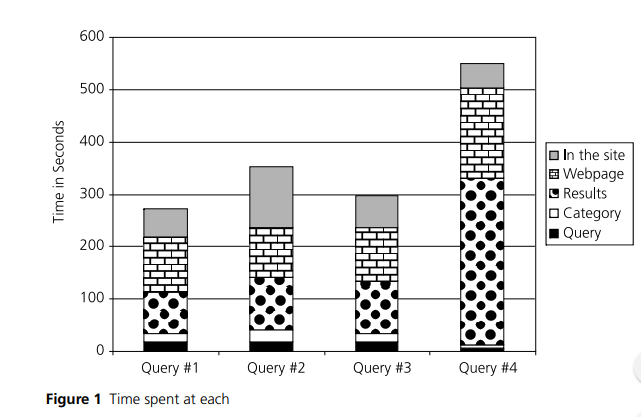
\includegraphics[width=0.8\textwidth]{Capture23.png}
	\caption{ Time spent at each stage \label{fig23}}
\end{figure}    

\textbf{Formulating queries and selecting categories}

For the first two tasks, participants have entered various queries to search for information for each topic and have also selected various categories. 12 participants have performed the Task 1 and 23 entries have been provided by these participants. However, for the Task 2 less variability in query content has been observed. 

Queries and categories for the Task 1 are shown in Figure~\ref{fig24}.

\begin{figure}[t!]
	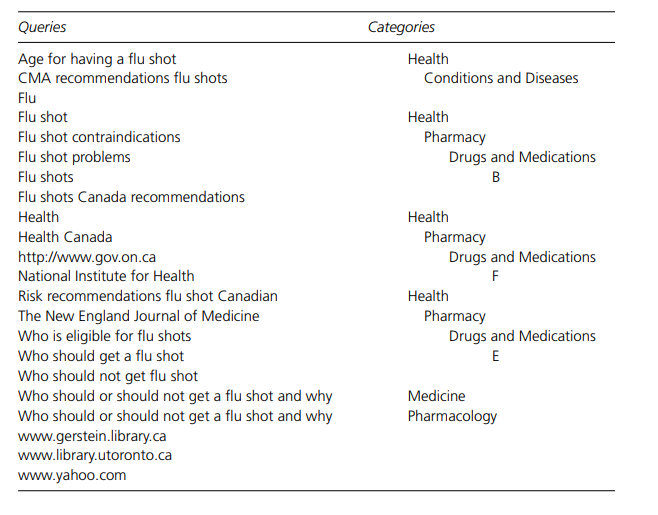
\includegraphics[width=0.8\textwidth]{Capture24.png}
	\caption{ Queries and categories for the Task 1 \label{fig24}}
\end{figure}            

Queries and categories for the Task 2 are shown in Figure~\ref{fig25}.

\begin{figure}[t!]
	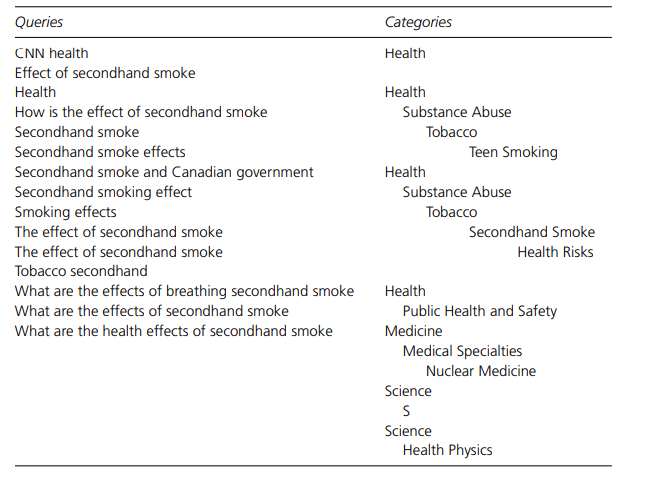
\includegraphics[width=0.8\textwidth]{Capture25.png}
	\caption{ Queries and categories for the Task 2 \label{fig25}}
\end{figure}  
    
The issues that participants have faced while constructing queries and category selection have been identified by the information gathered in post-search interviews. When considering query formulation, several processes have been used by the participants. The most popular method has been to use a keyword search either on a search engine or on a website of interest. It has also been identified that keyword search has been used as a ‘trial and error’ method by the participants.       

According to the observations, the participants have had a belief that when using keyword search they have a higher level of control over the search process and results because participants are able to choose their own search words. This has allowed them to define the search and refine it in a manner of their own choosing. For instance, according to one participant’s opinion adding specific words while searching, made it more ‘robust.’ Other participants have shown a behaviour to restrict their search by source of information. Some have also been concerned about the reliability of the source of information. Except these some other approaches, such as the preceding of search terms with a plus sign to ensure results fell within a common page and encapsulating search terms in quotation marks to ensure that all terms are found together in sites identified in the search results     have also been used while conducting keyword searches.            

Therefore, according to the observed results keyword search method has been preferred over the use of categories. Some participants have seen categories as an impediment to finding information rather than a useful form of assistance. In addition, categories have been identified as a less direct route to locate information because categories resulted in ‘more steps’. Also, the information contained in categories have been too general. Furthermore, the exposure to advertisements have been increased when using categories and the time taken to find the information being sought has also been identified as high.         

\textbf{Selecting from the results list}

On average 5.4 pages of results lists have been examined by the participants. The average rank on a results list page has been identified as 4 and therefore, all items on the results list page have had an equal likelihood of being selected. 

According to the information gathered from the post-search interviews, participants have reported a more methodical approach to determine which options to be chosen from the results list. The summaries and URLs provided have been used by the participants to select the most appropriate links to explore. Descriptions have been important because they have been used to determine whether a site’s information is matching with the perceived information needs and then to decide upon selection or de-selection of the site. The URL has also played an important role because it has helped to identify the nature of the site, such as whether it is an information-based site or an e-commerce site, and to assess the kind of information on the site. Titles have also been used as a source of information for selection.   
  
Except that other information, such as dates, size of the site, and type of file (e.g. PDF) have been least used as sources of information. A few participants have looked at the number of results on the results list. For instance, according to one participant a large number of results indicates that the search needed to be refined. In cases where there are a large number of results retrieved, participants have tended to jump to pages further down if the initial results did not appear to be relevant.
   
In addition, the URLs have been used to  assess the potential credibility of the information that has been found.

According to some participants  university, government, scientific, pharmaceutical research information and associations for medical professionals have been reliable sources. However, credibility has been identified as a subjective assessment because it has been dependent on participants' personal opinions and prior knowledge/ experience.

The rank order in which the results have been appeared on the results list, has not been considered by the participants as a criterion for determining appropriateness or credibility of the results. Participants have shown a behaviour where they have looked at links on several pages of the results list. Some participants have shown a behaviour of choosing the first link on the results list. The reasons for choosing the first link have been identified as because of the convenience as it is the quickest link to access and as a starting point in a process of trial and error.  

\textbf{Identifying appropriate websites} 

The average number of web
pages selected by the participants has been 2.6 web pages. Once they have identified a useful site, then they have further examined about another three web pages. 

According to the judges the average web page ‘aboutness’ has been 4.5 out of 5. All the pages which have been identified as relevant to the tasks, also have been assessed by a judge and a average score of 4.5 out of 5 has been assigned by the judges. Therefore, it is said that the pages which have been examined by participants are clearly on the topic of the search, and participants have been able to complete between 80-100\% of each task. Out of pages which have been identified as relevant 44\% have not had any advertisements and 40\% have been created by a government agency. The pages have been primarily classified as informational and followed by journal articles, fact sheets and newspaper articles. 

Once a link has been chosen from the results list, then the participants had to determine whether that link’s information satisfy their information needs. According to the post-search interviews’ information, the initial impressions and the subsequent use or rejection of the site, has involved at least one key consideration out of the three which have been identified.     

1. Information expectations: does the site provide any or all of the information being sought? 

2. Information quality: who is the author of the site and the information contained therein? What is the purpose of the site (e.g. to provide information, to sell products, to promote unsubstantiated opinions)? How is the information presented (e.g. opinion-based articles, discussion group, academic research, formal medical findings)? 

3. Information presentation and accessibility: how difficult is it to find the desired information on the site? Is the information easy to understand? 

It has been observed that sites which have been able to provide information that is being sought, have been considered as useful and the other sites which have not been able to satisfy information needs, have been rejected. The credibility of the sites has also been important when selecting a link from the results list. The credibility has been established by looking at factors which have been identified as representing information quality. Also, the participants have shown a behaviour of looking for recognizable authoritative sources (Centre for Disease Control) or sources with the appearance of authority (physicians).      

The motivation of the site and the way the information has been presented have also been important for the participants when determining the credibility. According to the information gathered participants have been disappointed with the sites which have aimed at selling products and presenting information in a less formal or authoritative manner.  

Another factor which has influenced participants when selecting and using sites is the ease of  finding and understanding information. Therefore, concise layouts with clear menus and elements, such as search boxes and bullets or titles to partition text have been identified as features which facilitated participants in finding information and encouraging the use of sites. Participants have shown a behaviour to reject sites with poor lay outs, too much technical information and pop-up or sidebar advertisements with unrelated information.  
              
\textbf{Analysis and discussion} 

According to the analysed results it has shown that participants are likely to perform keyword searches. However, the queries which have been issued have not always been immediately successful. When analysing different types of queries which have been issued and the time taken to issue queries, it has been noted that query formulation has been a quick, and sort of a trial and error process. In cases where participants have been asked to increase their query length, two problems have been identified. Firstly, participants have shown a reluctant behaviour to add to a few simple keywords and the search engines have often removed words that made a query meaningful to a user. Therefore, the system has limited the improvements that could be performed while constructing queries and the apparent system improvements have not been realized by the participants.        

Several factors, such as what participants have been looking for, their knowledge of the area, their biases in terms of credibility and their personal understanding of the topic have influenced keyword searches. When using the categories to search for information, participants have faced similar issues as they have faced when using keyword searches. The use of categories has also shown a trial and error behaviour. Having prior knowledge of the topic has been helpful when selecting categories. Not knowing what a category represents or contains has been identified as a barrier to use categories. In addition, having an endless set of category levels has been identified as not conducive to effective use. 

The results list has played a crucial role in tasks’ success. The results lists have been examined thoroughly by the participants before clicking on a link. Therefore, the participants have examined pages of results before even selecting the first link, in order to make sure that the target page is likely to be suitable and pertinent. Summaries for each result on several pages have been examined by the participants for its pertinence. When considering the time participants have taken to select from the results pages, it has been noted that the information design of the pages has had a significant barrier to the online health consumer.      

Participants have shown a behaviour to abandon pages quickly by considering several key components simultaneously. Participants sometimes have made erroneous decisions by considering the web page appearances. In addition, they have judged the authority of the pages based on layout and presentation of the pages.        

When selecting pages from results lists and selecting appropriate web pages, credibility and trust have been identified as key issues. As participants’ intention has been to find useful and pertinent information, they have not liked commercial sites or advertisements. However, it has been observed that approximately half of the pages which have been declared as pertinent have had advertisements on them. Participants have also been identified as concerned about the reliability and credibility of the sites and have worked hard to avoid unreliable sites. 

It has been observed that participants have been able to locate possible answers to the questions by putting some effort on finding them. The main challenges which have been identified are formulating good queries, and having a results list with appropriate design and standard which is more likely to enable easy scanning and efficient recognition.  

The solution for the identified issues which have been faced by the consumers is to design proper systems which will provide assistance to query development and which will evaluate the information that is being provided. Also, it has been identified that the key to successful queries lie on the terminological infrastructure which supports the search process. In addition, it is important for such an infrastructure to be flexible and responsive to the taken efforts by both laypersons and experts. 

Another challenge is identified when developing appropriate summaries. The results lists which have been used for this study have been consisted of large bibliographic databases and library catalogues so as to make it easier for the participants to scan a list of items quickly. Usually in search engines the use of summaries is extremely limited and rather KWIC style format is preferred. It is said that when considering consumer health information, the format and the content of the structure should be rethought with consumer in mind. It is also expected from these summaries on the results list to indicate the reliability and credibility of the documents that they represent and to alert the user about the type of site and information content.           

\textbf{Conclusions}

Both information design and search engine technology should be blended together in order to build good consumer health information systems. Also, the design of consumer health information systems should focus on their potential users and therefore, should reflect an understanding of users’ need for information and how they search for that information. The relevant components from these two perspectives (users’ need for information and how they search for that information) are expected to be incorporated into a framework. Such a framework can help to create appropriate information structures which will then support findability and use.

It has been observed that consumer health information search still remains as a challenging task for the average person. Health information is found to be voluminous, created by variety of people with various motivations and is accessed by users who have different comprehension levels, searching abilities and levels of information needs. Therefore, the challenge for researchers and system developers is to understand the method to structure information unwieldy and at the same time to make it intuitive.  

\section{Zuccon, G., \& Koopman, B. (2018, March). Choices in Knowledge-Base Retrieval for Consumer Health Search. In European Conference on Information Retrieval (pp. 72-85). Springer, Cham.}  

In this paper the researchers have focused on overcoming coming consumer health search problems by expanding/ reformulating health queries with more effective terms. Therefore, the aim of this research has been to investigate the use of specialised health knowledge bases (MeSH and UMLS) and general knowledge bases (Wikipedia) to expand consumer health queries by linking queries to entities in knowledge bases. The researchers have adopted the 'Entity Query Feature Expansion' model for their empirical evaluation. Researchers have also evaluated the impact of different choices in knowledge based retrieval for consumer health search, such as:

(i) Knowledge based construction
(ii) Entity mention extraction
(iii) Entity mapping
(iv) Source of expansion
(v) Use of relevance feedback

They have also investigated to identify whether the use of a specialised knowledge base is preferred over a general knowledge base.           

\textbf{Expansion Model}

As mentioned earlier 'Entity Query Feature Expansion' model has been used for this study for retrieval on both the Wikipedia and UMLS as the knowledge bases.  

Wikipedia KB: A single entity has been represented by a single Wikipedia page (page title identifies the entity). Other page features which have been useful for a retrieval scenario are entity title (E), categories (C), links (L), aliases (A), and body (B)

UMLS KB: A single entity has been represented by the most frequently used terms for a single concept unique identifier (CUI). Other features of a UMLS knowledge base entity have been aliases (A), body (B), parent concepts (P) and related concepts (R). 

The features which have been used for mapping the queries to entities in the knowledge bases and as the source of expansion terms are shown in Figure~\ref{fig26}.

\begin{figure}[t!]
	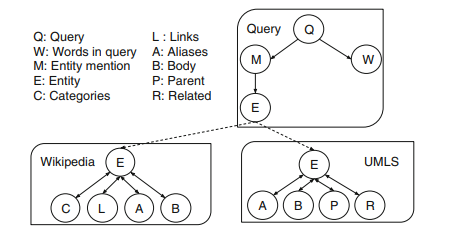
\includegraphics[width=0.8\textwidth]{Capture26.png}
	\caption{Summary of expansion sources \label{fig26}}
\end{figure}      

The defined query expansion model is shown in Figure~\ref{fig27}.

M: The entity mentions and contain uni-, bi-, and tri-gram generated from the query
f: A function used to extract the expansion terms
λf(0, 1): A weighting factor
ϑf(EM,SE): A function to map entity mention M to the
knowledge based features EM and  extract
expansion terms from source of expansion SE  
 

\begin{figure}[b!]
	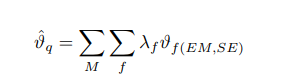
\includegraphics[width=0.8\textwidth]{Capture27.png}
	\caption{The defined expansion model \label{fig27}}
\end{figure}      

\textbf{ Choices in Knowledge Base Retrieval}

\textbf{3.1 Knowledge Base Construction} 

The researchers have had to decide upon which entities should be considered to form the basis of the knowledge bases. Because the focus has been on the consumer health search, health-related entities have been considered. For Wikipedia three choices have been made in order collect health related pages, such as:
    
(WC-Type): Pages with Medicine infobox type

(WC-TypeLinks) : Pages with Medicine infobox type and with links to medical terminologies such as Mesh and UMLS 

(WC-UMLS): Pages with title matching an UMLS entity  
 
The last method which has been used is ‘QuickUMLS’. This has been used to map Wikipedia page titles to the UMLS. If the mapping has been successful, then they have included such Wikipedia entities (pages) in the knowledge base.
  
For UMLS, two choices have been considered:

(UC-All): All entities 

(UCMed): Entities related to four key aspects of medical decision criteria, such as symptoms, diagnostic test, diagnoses and treatments

\textbf{3.2 Entity Mentions Extraction} 

This has been the process of identifying text from the query which can be mapped to entities. Three choices have been considered to extract entity mentions:

(ME-All): Include all uni-, bi- and tri-grams of the query (default choice)

(ME-CHV): Include only those uni-, bi- and tri-grams of the query which had matching entities in the Consumer Health Vocabulary 

(MEUMLS): Include only those uni-, bi- and tri-grams of the query which had matching entities in the UMLS (via QuickUMLS)
  
All three choices have been used for both Wikipedia and UMLS knowledge bases

\textbf{3.3 Entity Mapping}

The researchers have searched for exact matches between mentions and entities, and have mapped a mention to an entity if there is an exact match between them. For Wikipedia the considered choices have been:  

(WEM-Title): titles

(WEM-Aliases): aliases

(WEMLinks): links

(WEM-Body): the entire bodies of the Wikipedia pages

(WEM-Cat): categories

(WEM-All): all the previous sources (default choice)


For Wikipedia the considered choices have been: 
 
(UEM-Title): titles

(UEM-Aliases): aliases

(UEMBody): the entire UMLS concept description

(UEM-Parent): parents

(UEMRelated): related entities

(UEM-All): all the previous sources (default choice)

(UEM-QuickUmls): use QuickUMLS to obtain entity mappings

\textbf{3.4 Source of Expansion}


The researchers have selected the sources from the knowledge bases to use for drawing candidate terms for query expansion. Three choices have been explored:

(SE-Title): titles associated with the entities

(SE-Aliases): aliases associated with the entities

(SE-All): both titles and aliases (default choice)
 
These choices have been used for both the Wikipedia and UMLS.

\textbf{3.5 Relevance Feedback}

Both explicit relevance feedback (RF) and Pseudo Relevance Feedback (PRF) have been considered.
 
Explicit relevance feedback (RF) has been performed by extracting the ten most important health related words from each of the top three relevant documents (have used relevance labels). Therefore, this has resulted in a maximum of thirty expansion terms.

Pseudo Relevance Feedback (PRF) has been performed by extracting the ten most important health related words from the top three ranked documents (regardless of their relevance label). 

A term has been considered as health related if this term exactly matched with a title or an alias of an entity in the target knowledge base (Wikipedia or UMLS). 

\textbf{Empirical Evaluation}

The methods have been empirically evaluated using the CLEF 2016 eHealth, in order to identify whether there is any influence on query expansion for the consumer health search task by the choices of knowledge base retrieval. 300 query topics have been considered for this study. Documents have been taken from Clueweb12b13. The collection has been indexed using Elasticsearch 5.1.1, with stopping and stemming. The researchers have implemented a baseline using BM25F (allows to specify boosting factors for matches occurring in different fields of the indexed web page) with b = 0.75 and k1=1.2. For the purpose of this study the title field and the body field have been considered with boost factors as 1 and 3, respectively.        

Wikipedia knowledge base has been constructed using candidate pages from the English subset of Wikipedia. This knowledge base has been limited as to have current revisions only and without talk or user pages. The chosen candidate pages have been processed according to the different choices available for knowledge base construction. The chosen pages have also been indexed using field-based indexing. This has enabled the use of fields as a source of query expansion terms.     

UMLS knowledge base has been constructed by indexing 3,057,234 non-obsolete English terms with several fields, such as title, aliases, body, parent and related.

Results have been evaluated using nDCG@10 and RBP@10 according to the CLEF 2016 collection. The reason for this has been because when consumers’ search for health information they tend to primality examine the first few search results. The influence of unjudged documents on the evaluation has been reduced by using bpref. The superscripts of the results tables have been used to refer to statistical significance between the result and the result from the choice associated with the superscript. In addition, the researchers have recorded the average number of terms added in the expanded query (|exp|) and the number of expanded queries, queries with a gain for RBP@10, and a loss for RBP@10 as a triplet < e, g, l >.  

The researchers have empirically evaluated the influence each choice has had on retrieval effectiveness by examining each choice. This has been done for both knowledge bases in order to observe which knowledge base supports the best for consumer health search. A best setting has been fixed for each choice and has also been used for the subsequent choice. The best setting has been firstly decided using results for the all queries set. In cases where there has been no best method, then the researchers have checked results from the high coverage queries set.           

Influence of choices in knowledge base construction are shown in Figure~\ref{fig28}.

\begin{figure}[t!]
	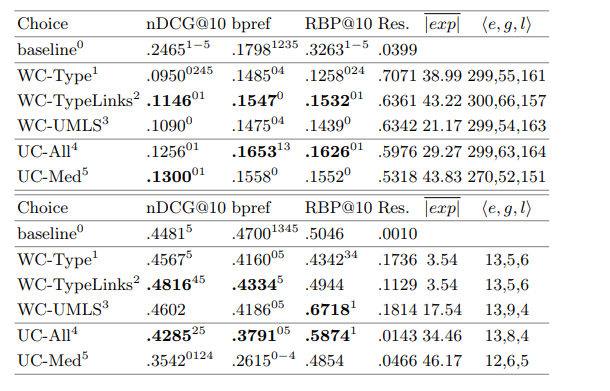
\includegraphics[width=0.8\textwidth]{Capture28.png}
	\caption{Influence of choices in knowledge base construction: all queries (top) and high coverage
		queries (bottom) \label{fig28}}
\end{figure} 

\textbf{4.1 Knowledge Base Construction}

The results for the influence of choices in knowledge base construction have been averaged over all 300 queries in the CLEF 2016 collection.   

According to the results:

Wikipedia knowledge base: The choice of WC-TypeLinks (infobox type and links to medical terminologies) has lead to the highest effectiveness across most measures

UMLS knowledge base: UC-All has lead to the higher effectiveness for all measures 

However, it has been observed that the baseline has performed considerably better than any of the knowledge base retrieval methods.

When considering the unjudged documents, knowledge base retrieval methods have ranked many unjudged documents amongst the top 10 results for a large number of queries. However, the baseline method has ranked much lower number of unjudged documents amongst the top 10. It has been observed that large values of RBP residuals are associated with the knowledge base retrieval methods when compared to the residuals of the baseline and therefore, it clearly influences the results. It is also said that in a case where all the unjudged documents are identified as relevant, the RBP@10 of the knowledge base retrieval methods would prove largely superior than that of the baseline (compare the residuals).

Then the researchers have considered a subset of queries which have had a maximum of 2 unjudged documents out of the first 10 documents. This threshold has been decided by examining the number of unjudged documents for the baseline method. This has produced a different subset of queries for each of the considered choices. It has been noted that these subsets have had the same average “coverage” with respect to the relevance assessments. These subsets have been called as ‘the high coverage queries’. This subset has consisted of 13 queries.  According to the results, there has been a reduction of the residuals, and a reduction of the gaps between knowledge base retrieval methods and the baselines. When considering the Wikipedia knowledge base, the trends in effectiveness across the considered choices have not been changed. Unlike the methods on the Wikipedia knowledge base, the relative effectiveness of the UMLS knowledge base method (UC-All) has shown to be less effective.   

According to the results of the Wikipedia knowledge base, the best setting has been identified as the WC-TypeLinks. Therefore, WC-TypeLinks has been used for the rest of the following analyses for Wikipedia knowledge base. UC-All has been used for the UMLS knowledge base.

\textbf{4.2 Entity Mentions Extraction} 

The results (top: 300 queries and bottom: 22 high coverage queries) obtained by comparing choices for entity mention extraction are shown in Figure~\ref{fig29}.

\begin{figure}[t!]
	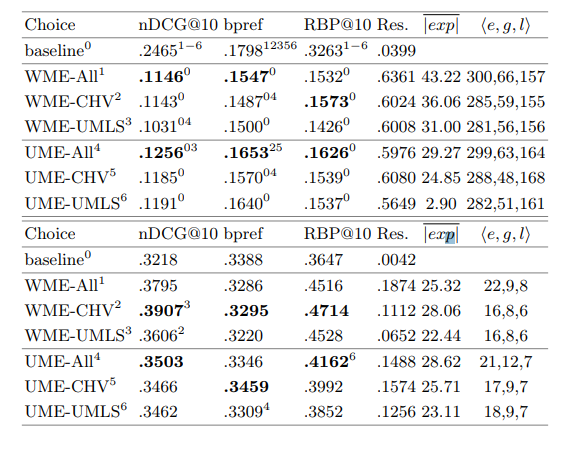
\includegraphics[width=0.8\textwidth]{Capture29.png}
	\caption{Influence of choices in entity mention extraction; all queries (top), high coverage queries (bottom) \label{fig29}}
\end{figure}  

According to the results of the Wikipedia knowledge base, the choice of constructing entity mentions with uni-, bi- and tri-grams of the queries that matched CHV (WME-CHV) has shown to be the one that provided the highest retrieval effectiveness. This result has been clearly shown for the high coverage set. However, when considering the ‘all queries set’, the difference between (WME-CHV) strategy and using all grams (WME-All) strategy has not shown a clear result. Therefore, the researchers have concluded that WME-CHV strategy as the most effective choice and have selected WME-CHV to be used in the remaining analyses. 

For UMLS knowledge base, results have showed that constructing entity mentions using all uni-, bi-, and tri-grams of the queries (UME-ALL) terms are able to provide the highest retrieval effectiveness. Therefore, the researchers have selected UME-ALL to be used in the remaining analyses.  

\textbf{4.3 Entity Mapping}   

The results (top: 300 queries and bottom: 22 high coverage queries) obtained by comparing choices for entity mapping are shown in Figure~\ref{fig30}.  

\begin{figure}[t!]
	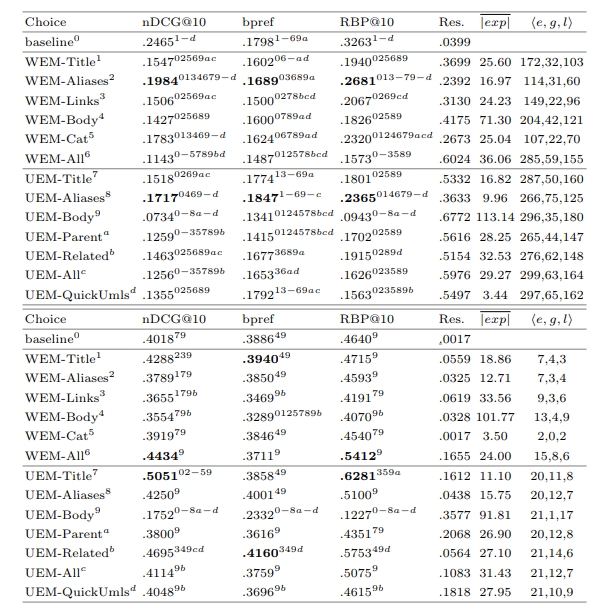
\includegraphics[width=0.8\textwidth]{Capture30.png}
	\caption{Influence of choices in entity mapping; all queries (top), high coverage queries (bottom) \label{fig30}}
\end{figure} 

According to the results of the two knowledge bases mapping entities to Aliases (WEM-Aliases and UEM-Aliases) have outperformed the other approaches (all queries). However, the results for the high coverage queries have shown mixed results. Therefore, the researchers have selected WEM-Aliases and UEM-Aliases to be used for the subsequent analyses.

\textbf{4.4 Source of Expansion} 

The results (top: 300 queries and bottom: 119 high coverage queries) obtained by comparing scores of query expansion are shown in Figure~\ref{fig31}. 

\begin{figure}[b!]
	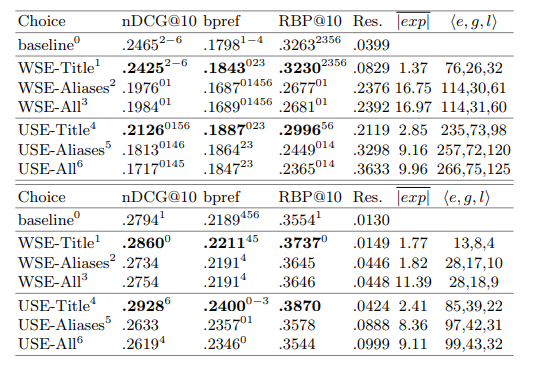
\includegraphics[width=0.8\textwidth]{Capture31.png}
	\caption{Influence of choices in source of expansion; all queries (top), high coverage queries (bottom) \label{fig31}}
\end{figure} 

According to the observed results, for both the knowledge bases (Wikipedia and UMLS), the selection of titles as the source of expansion (WSE-Title and USE-Title) has shown to be the most effective choice when compared to other choices. Therefore, the researchers have selected WSE-Title and USE-Title to be used for the subsequent analyses.    

\textbf{4.5 Relevance Feedback} 

The results (top: 300 queries and bottom: 80 high coverage queries) obtained with and without relevance feedback are shown in Figure~\ref{fig32}. 

\begin{figure}[t!]
	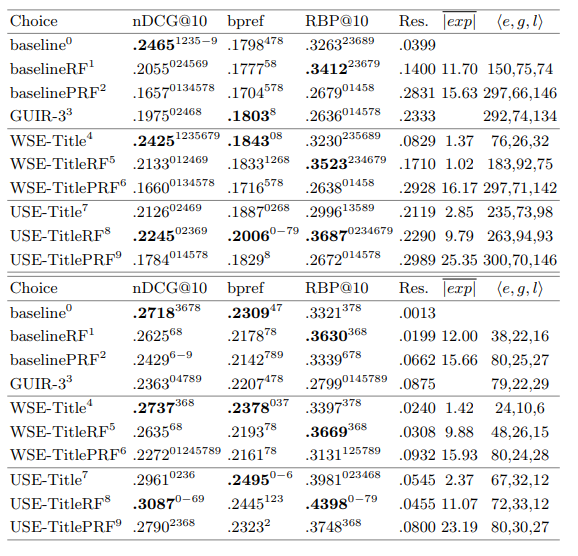
\includegraphics[width=0.8\textwidth]{Capture32.png}
	\caption{Influence of choices in relevance feedback; all queries (top), high coverage queries (bottom) \label{fig32}}
\end{figure} 

When considering results for Wikipedia it has been noted that the addition of feedback has produced mixed results. RF has been able to produce the best RBP@10 across all types of queries. The Wikipedia WSETitle choice has been able to perform better without the addition of feedback in terms of nDCG@10 and bpref. When considering results for UMLS, it has been noted that RF has been able to produce the best performance for all queries set on all measures. When observing the results for high coverage queries, it has been identified that the USE-Title obtained better bpref without the addition of relevance feedback. For the baseline method, the application of relevance feedback has only improved RBP@10 when using true relevance information (RF). Therefore, it has been observed that the baseline method has performed worse when compared to the knowledge base methods.               

\textbf{Further Analysis and Discussion} 

According to the analysis of the results researchers have found that:

1.	PRF does not improve results, independently of the knowledge base

2.	RF provide improved effectiveness. UMLS-based best settings (USE-TitleRF) has provided generally better improved effectiveness when compared to Wikipedia-based best settings (WSE-TitleRF) for both all queries and the high coverage queries sets

3.	When considering high coverage queries set, as independent of the relevance feedback’s application, UMLS based knowledge base’s best settings have been more effective than Wikipedia based knowledge base settings. When considering all queries set, UMLS based knowledge base settings with RF has performed better than Wikipedia based knowledge base settings on all measures

4.	UMLS knowledge base has expanded more queries than the Wikipedia knowledge base. This is due to the reason that the Wikipedia’s knowledge base is comparatively incomplete because it has considered only pages with health infobox and links to medical terms. 

In addition, according to the analysis it has been identified that the two methods have provided different query expansions where on average they have had only 8.9\% of common expansion terms. It has also been noticed that the two methods have retrieved different sets of documents (average overlap for the best settings without relevance feedback has been 61\% of the top 1,000 (10) documents). 

The researchers have contextualise the results obtained using knowledge base retrieval methods by reporting the results of the method implemented by the GUIR-3 submission to the CLEF 2016 challenge. This has been the best performing, comparable query expansion method at CLEF 2016. Basically, this method has expanded queries by mapping query entities to the UMLS, and navigating the UMLS tree to gather hypernims from mapped entities as source of expansion. Unlike the original method, this study has relied on BM25F rather than DFR as scoring method and QuickUMLS in place of Metamap. Because of this the researchers have been able to directly compare with the baseline method and knowledge base retrieval methods.    

When analysing the number of expansion terms added across the knowledge base methods, the researchers have identified that the effective choices for knowledge base query expansion has lead to produce the lowest number of expansion terms (as well as expanding the smallest number of queries). Relevance feedback has added a significant number of expansion terms (as well as expanding a large number of queries). PRF has been identified as adding expansion terms in a more aggressive manner. Because of this reason RF, which has shown a more conservative behaviour in both queries that are expanded and the extent of expansion, has outperformed PRF.  

Researchers have also examined the impact of query expansion for each query by analysing the results.  

The gains/losses vs. baseline obtained by the best settings of Wikipedia knowledge base (WSE-TitleRF) and UMLS knowledge base (USE-TitleRF) are shown in Figure~\ref{fig33}.

\begin{figure}[b!]
	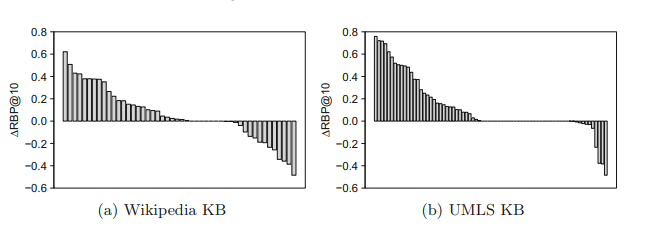
\includegraphics[width=0.8\textwidth]{Capture33.png}
	\caption{Changes in RBP@10 between the Entity Query Feature Expansion model utilising the best settings vs. baseline \label{fig33}}
\end{figure} 

In total, for WSE-TitleRF (USE-TitleRF), 183 queries have been expanded by the model (48 in the high coverage set). Out of these query expansions, 16 have shown no change in effectiveness when compared to the baseline (7 in the high coverage set). When considering the remaining query expansions, 92 have shown improvements (26 in the high coverage) and 75 have shown losses (15 in the high coverage). These improvements/losses have been measured using RBP@10 and therefore, expanded queries with low coverage have been identified as unlikely to perform as effective as expanded queries with high coverage.    

\textbf{Conclusions} 

This study has explored the influence of different choices in knowledge base retrieval for consumer health search. The choices have included knowledge base construction, entity mentions extraction, entity mapping, source of expansion, and relevance feedback. The researchers have compared the effectiveness of Wikipedia as a general knowledge base and UMLS as a medical specialised knowledge base as the basis for query expansion. According to the evaluation results the best settings for the Wikipedia knowledge base have been identified as: (1) indexing only Wikipedia pages that have health related infobox types or links to medical terminologies, (2) using uni-, bi-, and tri-grams of the original queries that matched CHV terms as entity mentions, (3) mapping entity mentions to Wikipedia entities based on the Aliases feature, (4) using source expansion terms from the mapped Wikipedia page Title, and (5) adding relevance feedback terms. The best settings for the UMLS knowledge base have been identified as: (1) indexing all UMLS concepts, (2) using all uni-, bi-, and tri-grams of the original queries as entity mentions, (3) mapping entity mentions to UMLS entities based on the Aliases feature, (4) using source expansion terms from the mapped UMLS Title feature, and (5) adding relevance feedback terms.    

The results have been analysed after tuning the five choices. These results have shown that overall, UMLS based knowledge base settings have been more effective when compared to Wikipedia based knowledge base settings.  When considering all queries set, the best UMLS knowledge base settings (USE-TitleRF) have performed better than the baseline in terms of bpref (+11.56\%) and RBP@10 (+12.99\%). When considering queries with high coverage of judged documents, USE-TitleRF has been more effective for a majority of queries and has outperformed the baseline on all measures, such as nDCG@10 (+12.58\%), bpref (+5.89\%), and RBP@10 (+32.43\%). According to these results the researchers have confirmed that the use of a knowledge-base retrieval approach has the ability to translate well into this challenging consumer health search domain.                   

\textbf{Limitations}

The number of unjudged documents retrieved using the expanded queries on the CLEF 2016 collection, has been identified as the major limitation of this study. Researchers have tried to mitigate this by considering bpref, RBP and RBP residuals. However, still the researchers have found it challenging to fairly evaluate the methods. Nevertheless, this investigation of choices in knowledge base retrieval for consumer health search has been able to highlight both pitfalls and payoffs.
 
\end{document} 